\documentclass{article}\usepackage[]{graphicx}\usepackage[]{xcolor}
% maxwidth is the original width if it is less than linewidth
% otherwise use linewidth (to make sure the graphics do not exceed the margin)
\makeatletter
\def\maxwidth{ %
  \ifdim\Gin@nat@width>\linewidth
    \linewidth
  \else
    \Gin@nat@width
  \fi
}
\makeatother

\definecolor{fgcolor}{rgb}{0.345, 0.345, 0.345}
\newcommand{\hlnum}[1]{\textcolor[rgb]{0.686,0.059,0.569}{#1}}%
\newcommand{\hlsng}[1]{\textcolor[rgb]{0.192,0.494,0.8}{#1}}%
\newcommand{\hlcom}[1]{\textcolor[rgb]{0.678,0.584,0.686}{\textit{#1}}}%
\newcommand{\hlopt}[1]{\textcolor[rgb]{0,0,0}{#1}}%
\newcommand{\hldef}[1]{\textcolor[rgb]{0.345,0.345,0.345}{#1}}%
\newcommand{\hlkwa}[1]{\textcolor[rgb]{0.161,0.373,0.58}{\textbf{#1}}}%
\newcommand{\hlkwb}[1]{\textcolor[rgb]{0.69,0.353,0.396}{#1}}%
\newcommand{\hlkwc}[1]{\textcolor[rgb]{0.333,0.667,0.333}{#1}}%
\newcommand{\hlkwd}[1]{\textcolor[rgb]{0.737,0.353,0.396}{\textbf{#1}}}%
\let\hlipl\hlkwb

\usepackage{framed}
\makeatletter
\newenvironment{kframe}{%
 \def\at@end@of@kframe{}%
 \ifinner\ifhmode%
  \def\at@end@of@kframe{\end{minipage}}%
  \begin{minipage}{\columnwidth}%
 \fi\fi%
 \def\FrameCommand##1{\hskip\@totalleftmargin \hskip-\fboxsep
 \colorbox{shadecolor}{##1}\hskip-\fboxsep
     % There is no \\@totalrightmargin, so:
     \hskip-\linewidth \hskip-\@totalleftmargin \hskip\columnwidth}%
 \MakeFramed {\advance\hsize-\width
   \@totalleftmargin\z@ \linewidth\hsize
   \@setminipage}}%
 {\par\unskip\endMakeFramed%
 \at@end@of@kframe}
\makeatother

\definecolor{shadecolor}{rgb}{.97, .97, .97}
\definecolor{messagecolor}{rgb}{0, 0, 0}
\definecolor{warningcolor}{rgb}{1, 0, 1}
\definecolor{errorcolor}{rgb}{1, 0, 0}
\newenvironment{knitrout}{}{} % an empty environment to be redefined in TeX

\usepackage{alltt}
\usepackage[sc]{mathpazo}
\renewcommand{\sfdefault}{lmss}
\renewcommand{\ttdefault}{lmtt}
\usepackage[T1]{fontenc}
\usepackage{geometry}
\geometry{verbose,tmargin=2.5cm,bmargin=2.5cm,lmargin=2.5cm,rmargin=2.5cm}
\setcounter{secnumdepth}{2}
\setcounter{tocdepth}{2}
\usepackage[unicode=true,pdfusetitle,
 bookmarks=true,bookmarksnumbered=true,bookmarksopen=true,bookmarksopenlevel=2,
 breaklinks=false,pdfborder={0 0 1},backref=false,colorlinks=false]
 {hyperref}
\hypersetup{
 pdfstartview={XYZ null null 1}}

\makeatletter
%%%%%%%%%%%%%%%%%%%%%%%%%%%%%% User specified LaTeX commands.
\renewcommand{\textfraction}{0.05}
\renewcommand{\topfraction}{0.8}
\renewcommand{\bottomfraction}{0.8}
\renewcommand{\floatpagefraction}{0.75}

\makeatother
\IfFileExists{upquote.sty}{\usepackage{upquote}}{}
\begin{document}









\begin{knitrout}
\definecolor{shadecolor}{rgb}{0.969, 0.969, 0.969}\color{fgcolor}\begin{kframe}
\begin{alltt}
\hlcom{# This R script runs with a renv environment available in a dedicated Github Repository.}
\hlcom{# Below are the commands to recreate that environment in case the renv files were missing.}
\hlcom{#install.packages(renv)}
\hlcom{#renv::init()}
\hlcom{#renv::install("languageserver")}
\hlcom{#renv::install("httpgd")}
\hlcom{#renv::install("jsonlite")}
\hlcom{#renv::install("MASS")}
\hlcom{#renv::snapshot()}
\hldef{renv}\hlopt{::}\hlkwd{restore}\hldef{()}
\end{alltt}
\begin{verbatim}
## - The library is already synchronized with the lockfile.
\end{verbatim}
\begin{alltt}
\hlcom{################################################}
\hlcom{# (a)}

\hlcom{# Set the model's parameters a priori}
\hldef{rho}           \hlkwb{<-} \hlnum{0.9}
\hldef{sigma_epsilon} \hlkwb{<-} \hlnum{0.1}
\hldef{beta0}         \hlkwb{<-} \hlnum{4}
\hldef{beta1}         \hlkwb{<-} \hlnum{5}
\hldef{alpha0}        \hlkwb{<-} \hlopt{-}\hlnum{12} \hlcom{# Will be tuned later.}
\hldef{alpha1}        \hlkwb{<-} \hlnum{1}
\hldef{alpha2}        \hlkwb{<-} \hlnum{1}

\hlcom{# Generate Ei}
\hlkwd{set.seed}\hldef{(}\hlnum{202410041}\hldef{)}
\hldef{Ei} \hlkwb{<-} \hlkwd{round}\hldef{(}\hlkwd{abs}\hldef{(}\hlkwd{rnorm}\hldef{(}\hlnum{100000}\hldef{,} \hlnum{9}\hldef{,} \hlnum{5}\hldef{)))}

\hlcom{# Generate Zi}
\hlkwd{set.seed}\hldef{(}\hlnum{202410042}\hldef{)}
\hldef{Zi} \hlkwb{<-} \hlkwd{rnorm}\hldef{(}\hlnum{100000}\hldef{,} \hlnum{3}\hldef{,} \hlnum{0.75}\hldef{)}

\hlcom{# Generate error terms:}
\hlkwd{set.seed}\hldef{(}\hlnum{202410043}\hldef{)}
\hlkwd{library}\hldef{(MASS)}
\hldef{ui1_ui2} \hlkwb{<-} \hlkwd{mvrnorm}\hldef{(}
           \hlkwc{n} \hldef{=} \hlnum{100000}\hldef{,}
           \hlkwc{mu} \hldef{=} \hlkwd{c}\hldef{(}\hlnum{0}\hldef{,} \hlnum{0}\hldef{),}
           \hlkwc{Sigma} \hldef{=} \hlkwd{matrix}\hldef{(}\hlkwd{c}\hldef{(sigma_epsilon}\hlopt{^}\hlnum{2}\hldef{, rho}\hlopt{*}\hldef{sigma_epsilon, rho}\hlopt{*}\hldef{sigma_epsilon,} \hlnum{1}\hldef{),}
                          \hlkwc{ncol} \hldef{=} \hlnum{2}\hldef{)}
                  \hldef{)}

\hlcom{# Compute Wi}
\hldef{Wi} \hlkwb{<-} \hldef{beta0}\hlopt{+}\hldef{beta1}\hlopt{*}\hldef{Ei}\hlopt{+}\hldef{ui1_ui2[,}\hlnum{1}\hldef{]}

\hlcom{# "Fine tune" alpha0 such that the participation condition is met by exactly half of the data}
\hldef{participation_condition} \hlkwb{<-} \hldef{alpha0}\hlopt{+}\hldef{alpha1}\hlopt{*}\hldef{Ei}\hlopt{+}\hldef{alpha2}\hlopt{*}\hldef{Zi}\hlopt{+}\hldef{ui1_ui2[,}\hlnum{2}\hldef{]}
\hlkwd{length}\hldef{(participation_condition[participation_condition}\hlopt{>}\hlnum{0}\hldef{])}
\end{alltt}
\begin{verbatim}
## [1] 50217
\end{verbatim}
\begin{alltt}
\hlcom{# We can see that, with this value of alpha0 there are too many observations that satisfy}
\hlcom{#the participation condition.}
\hlkwa{while} \hldef{(}\hlkwd{length}\hldef{(participation_condition[participation_condition}\hlopt{>}\hlnum{0}\hldef{])}\hlopt{>}\hlnum{50000}\hldef{) \{}
   \hldef{alpha0} \hlkwb{<-} \hldef{alpha0}\hlopt{-}\hlnum{0.00001}
   \hldef{participation_condition} \hlkwb{<-} \hldef{alpha0}\hlopt{+}\hldef{alpha1}\hlopt{*}\hldef{Ei}\hlopt{+}\hldef{alpha2}\hlopt{*}\hldef{Zi}\hlopt{+}\hldef{ui1_ui2[,}\hlnum{2}\hldef{]}
   \hlkwd{print}\hldef{(alpha0)}
   \hlkwd{print}\hldef{(}\hlkwd{length}\hldef{(participation_condition[participation_condition}\hlopt{>}\hlnum{0}\hldef{]))}
\hldef{\}}
\end{alltt}
\begin{verbatim}
## [1] -12.00001
## [1] 50217
[...]
## [1] -12.03037
## [1] 50000
\end{verbatim}
\begin{alltt}
\hlcom{# We get alpha0=-12.03037. Explicitely set alpha0 accordingly:}
\hldef{alpha0} \hlkwb{<-} \hlopt{-}\hlnum{12.03037}
\hldef{participation_condition} \hlkwb{<-} \hldef{alpha0}\hlopt{+}\hldef{alpha1}\hlopt{*}\hldef{Ei}\hlopt{+}\hldef{alpha2}\hlopt{*}\hldef{Zi}\hlopt{+}\hldef{ui1_ui2[,}\hlnum{2}\hldef{]}
\hlkwd{length}\hldef{(participation_condition[participation_condition}\hlopt{>}\hlnum{0}\hldef{])}
\end{alltt}
\begin{verbatim}
## [1] 50000
\end{verbatim}
\begin{alltt}
\hlcom{# Create Wi_observed and dummy participate according to the participation decision model}
\hldef{Wi_observed} \hlkwb{<-} \hldef{Wi}
\hldef{participate} \hlkwb{<-} \hldef{Wi}\hlopt{/}\hldef{Wi}
\hlkwa{for} \hldef{(i} \hlkwa{in} \hlnum{1}\hlopt{:}\hlkwd{length}\hldef{(participation_condition))}
\hldef{\{}
  \hlkwa{if} \hldef{(participation_condition[i]}\hlopt{<=}\hlnum{0}\hldef{) \{Wi_observed[i]} \hlkwb{<-}\hlnum{NA}\hldef{\}}
  \hlkwa{if} \hldef{(participation_condition[i]}\hlopt{<=}\hlnum{0}\hldef{) \{participate[i]} \hlkwb{<-}\hlnum{0}\hldef{\}}
\hldef{\}}

\hlcom{# Computes the inverse Mills ratio derived from the participation decision model}
\hldef{inverse_mills_ratio} \hlkwb{<-} \hlkwd{dnorm}\hldef{((alpha0}\hlopt{+}\hldef{alpha1}\hlopt{*}\hldef{Ei}\hlopt{+}\hldef{alpha2}\hlopt{*}\hldef{Zi))}\hlopt{/}\hldef{(}\hlkwd{pnorm}\hldef{((alpha0}\hlopt{+}\hldef{alpha1}\hlopt{*}\hldef{Ei}\hlopt{+}\hldef{alpha2}\hlopt{*}\hldef{Zi)))}

\hlcom{# Create the dataset}
\hldef{dataset} \hlkwb{<-} \hlkwd{data.frame}\hldef{(}\hlkwc{Wi}\hldef{=Wi,}\hlkwc{Wi_observed}\hldef{=Wi_observed,}\hlkwc{participate}\hldef{=participate,}\hlkwc{Ei}\hldef{=Ei,}\hlkwc{Zi}\hldef{=Zi,}
                      \hlkwc{ui1}\hldef{=ui1_ui2[,}\hlnum{1}\hldef{],}\hlkwc{ui2}\hldef{=ui1_ui2[,}\hlnum{2}\hldef{],}
                      \hlkwc{participation_condition}\hldef{=participation_condition,}
                      \hlkwc{inverse_mills_ratio}\hldef{=inverse_mills_ratio)}

\hlcom{# Estimate the parameters of the three regressions}
\hldef{true_model} \hlkwb{<-} \hlkwd{lm}\hldef{(Wi}\hlopt{~}\hldef{Ei,} \hlkwc{data}\hldef{=dataset)}
\hlkwd{summary}\hldef{(true_model)}
\end{alltt}
\begin{verbatim}
## 
## Call:
## lm(formula = Wi ~ Ei, data = dataset)
## 
## Residuals:
##      Min       1Q   Median       3Q      Max 
## -0.45069 -0.06685  0.00023  0.06730  0.46423 
## 
## Coefficients:
##              Estimate Std. Error t value Pr(>|t|)    
## (Intercept) 3.9996045  0.0006857    5833   <2e-16 ***
## Ei          5.0000334  0.0000664   75301   <2e-16 ***
## ---
## Signif. codes:  0 '***' 0.001 '**' 0.01 '*' 0.05 '.' 0.1 ' ' 1
## 
## Residual standard error: 0.1001 on 99998 degrees of freedom
## Multiple R-squared:      1,	Adjusted R-squared:      1 
## F-statistic: 5.67e+09 on 1 and 99998 DF,  p-value: < 2.2e-16
\end{verbatim}
\begin{alltt}
\hldef{model_those_participating} \hlkwb{<-} \hlkwd{lm}\hldef{(Wi_observed}\hlopt{~}\hldef{Ei,} \hlkwc{data}\hldef{=dataset)}
\hlkwd{summary}\hldef{(model_those_participating)}
\end{alltt}
\begin{verbatim}
## 
## Call:
## lm(formula = Wi_observed ~ Ei, data = dataset)
## 
## Residuals:
##      Min       1Q   Median       3Q      Max 
## -0.37495 -0.06547 -0.00046  0.06562  0.43493 
## 
## Coefficients:
##              Estimate Std. Error t value Pr(>|t|)    
## (Intercept) 4.0830573  0.0018275    2234   <2e-16 ***
## Ei          4.9946553  0.0001374   36359   <2e-16 ***
## ---
## Signif. codes:  0 '***' 0.001 '**' 0.01 '*' 0.05 '.' 0.1 ' ' 1
## 
## Residual standard error: 0.09757 on 49998 degrees of freedom
##   (50000 observations deleted due to missingness)
## Multiple R-squared:      1,	Adjusted R-squared:      1 
## F-statistic: 1.322e+09 on 1 and 49998 DF,  p-value: < 2.2e-16
\end{verbatim}
\begin{alltt}
\hldef{model_those_participating_control} \hlkwb{<-} \hlkwd{lm}\hldef{(Wi_observed}\hlopt{~}\hldef{Ei}\hlopt{+}\hldef{inverse_mills_ratio,} \hlkwc{data}\hldef{=dataset)}
\hlkwd{summary}\hldef{(model_those_participating_control)}
\end{alltt}
\begin{verbatim}
## 
## Call:
## lm(formula = Wi_observed ~ Ei + inverse_mills_ratio, data = dataset)
## 
## Residuals:
##      Min       1Q   Median       3Q      Max 
## -0.36271 -0.06271 -0.00188  0.06227  0.39914 
## 
## Coefficients:
##                      Estimate Std. Error  t value Pr(>|t|)    
## (Intercept)         4.0001664  0.0022322  1791.99   <2e-16 ***
## Ei                  4.9999960  0.0001592 31403.78   <2e-16 ***
## inverse_mills_ratio 0.0903323  0.0014909    60.59   <2e-16 ***
## ---
## Signif. codes:  0 '***' 0.001 '**' 0.01 '*' 0.05 '.' 0.1 ' ' 1
## 
## Residual standard error: 0.09418 on 49997 degrees of freedom
##   (50000 observations deleted due to missingness)
## Multiple R-squared:      1,	Adjusted R-squared:      1 
## F-statistic: 7.095e+08 on 2 and 49997 DF,  p-value: < 2.2e-16
\end{verbatim}
\begin{alltt}
\hlcom{# Interpret the regression parameters and the direction of the bias (see copy)}

\hlcom{################################################}
\hlcom{# (b)}

\hlcom{# Estimate with probit the participation decision model:}
\hldef{participation_decision} \hlkwb{<-} \hlkwd{glm}\hldef{(participate}\hlopt{~}\hldef{Ei}\hlopt{+}\hldef{Zi,}\hlkwc{data} \hldef{= dataset,}\hlkwc{family} \hldef{=} \hlkwd{binomial}\hldef{(}\hlkwc{link} \hldef{= probit))}
\end{alltt}


{\ttfamily\noindent\color{warningcolor}{\#\# Warning: glm.fit: fitted probabilities numerically 0 or 1 occurred}}\begin{alltt}
\hldef{participation_probability} \hlkwb{<-} \hlkwd{predict}\hldef{(participation_decision,dataset,}\hlkwc{type}\hldef{=}\hlsng{"response"}\hldef{)}
\hldef{dataset} \hlkwb{<-} \hlkwd{data.frame}\hldef{(}\hlkwc{Wi}\hldef{=Wi,}\hlkwc{Wi_observed}\hldef{=Wi_observed,}\hlkwc{participate}\hldef{=participate,}\hlkwc{Ei}\hldef{=Ei,}\hlkwc{Zi}\hldef{=Zi,}
                      \hlkwc{ui1}\hldef{=ui1_ui2[,}\hlnum{1}\hldef{],}\hlkwc{ui2}\hldef{=ui1_ui2[,}\hlnum{2}\hldef{],}
                      \hlkwc{participation_condition}\hldef{=participation_condition,}
                      \hlkwc{inverse_mills_ratio}\hldef{=inverse_mills_ratio,}
                      \hlkwc{participation_probability}\hldef{=participation_probability)}

\hlcom{# Draw the plots:}
\hlkwd{plot}\hldef{(inverse_mills_ratio}\hlopt{~}\hldef{participation_probability,} \hlkwc{data}\hldef{=dataset)}
\end{alltt}
\end{kframe}

{\centering \includegraphics[width=.6\linewidth]{figure/script-Rnwauto-report-1} 

}


\begin{kframe}\begin{alltt}
\hlkwd{plot}\hldef{(inverse_mills_ratio}\hlopt{~}\hldef{participation_probability,} \hlkwc{data}\hldef{=}\hlkwd{subset}\hldef{(dataset,}
                                                    \hldef{alpha0}\hlopt{+}\hldef{alpha1}\hlopt{*}\hldef{Ei}\hlopt{+}\hldef{alpha2}\hlopt{*}\hldef{Zi}\hlopt{+}\hldef{ui1_ui2[,}\hlnum{2}\hldef{]}\hlopt{>}\hlnum{0}\hldef{))}

\hlcom{# Discuss the non-linearity of the inverse Mills ratio (see copy).}

\hlcom{################################################}
\hlcom{# (c)}

\hlcom{# Draw the best fit line for the sample of those who participate:}
\hldef{best_fit_line_participants} \hlkwb{<-} \hlkwd{lm}\hldef{(inverse_mills_ratio}\hlopt{~}\hldef{participation_probability,}
                                 \hlkwc{data}\hldef{=}\hlkwd{subset}\hldef{(dataset,}
                                 \hldef{alpha0}\hlopt{+}\hldef{alpha1}\hlopt{*}\hldef{Ei}\hlopt{+}\hldef{alpha2}\hlopt{*}\hldef{Zi}\hlopt{+}\hldef{ui1_ui2[,}\hlnum{2}\hldef{]}\hlopt{>}\hlnum{0}\hldef{))}
\hlkwd{plot}\hldef{(inverse_mills_ratio}\hlopt{~}\hldef{participation_probability,} \hlkwc{data}\hldef{=}\hlkwd{subset}\hldef{(dataset,}
                                                    \hldef{alpha0}\hlopt{+}\hldef{alpha1}\hlopt{*}\hldef{Ei}\hlopt{+}\hldef{alpha2}\hlopt{*}\hldef{Zi}\hlopt{+}\hldef{ui1_ui2[,}\hlnum{2}\hldef{]}\hlopt{>}\hlnum{0}\hldef{))}
\hlkwd{abline}\hldef{(}\hlkwc{a}\hldef{=}\hlkwd{coef}\hldef{(best_fit_line_participants)[}\hlnum{1}\hldef{],} \hlkwc{b}\hldef{=}\hlkwd{coef}\hldef{(best_fit_line_participants)[}\hlnum{2}\hldef{])}
\end{alltt}
\end{kframe}

{\centering 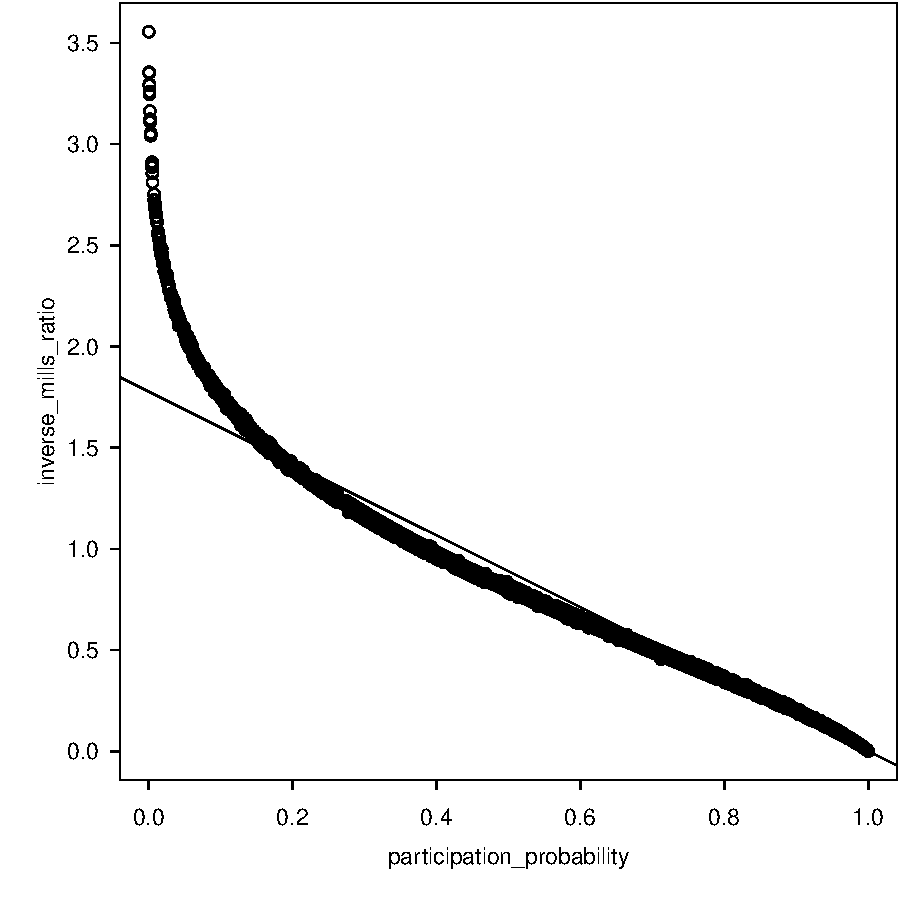
\includegraphics[width=.6\linewidth]{figure/script-Rnwauto-report-2} 

}


\begin{kframe}\begin{alltt}
\hlcom{# Draw the best fit line for the full sample.}
\hldef{best_fit_line_full_sample} \hlkwb{<-} \hlkwd{lm}\hldef{(inverse_mills_ratio}\hlopt{~}\hldef{participation_probability,} \hlkwc{data}\hldef{=dataset)}
\hlkwd{plot}\hldef{(inverse_mills_ratio}\hlopt{~}\hldef{participation_probability,} \hlkwc{data}\hldef{=dataset)}
\hlkwd{abline}\hldef{(}\hlkwc{a}\hldef{=}\hlkwd{coef}\hldef{(best_fit_line_full_sample)[}\hlnum{1}\hldef{],} \hlkwc{b}\hldef{=}\hlkwd{coef}\hldef{(best_fit_line_full_sample)[}\hlnum{2}\hldef{])}
\end{alltt}
\end{kframe}

{\centering \includegraphics[width=.6\linewidth]{figure/script-Rnwauto-report-3} 

}


\begin{kframe}\begin{alltt}
\hlcom{#Write a brief description (see copy).}

\hlcom{################################################}
\hlcom{# (d)}

\hlcom{# Attach all of your code.}
\end{alltt}
\end{kframe}
\end{knitrout}

The R session information (including the OS info, R version and all
packages used):

\begin{knitrout}
\definecolor{shadecolor}{rgb}{0.969, 0.969, 0.969}\color{fgcolor}\begin{kframe}
\begin{alltt}
\hlkwd{sessionInfo}\hldef{()}
\end{alltt}
\begin{verbatim}
## R version 4.3.2 (2023-10-31)
## Platform: aarch64-apple-darwin20 (64-bit)
## Running under: macOS Sonoma 14.4
## 
## Matrix products: default
## BLAS:   /Library/Frameworks/R.framework/Versions/4.3-arm64/Resources/lib/libRblas.0.dylib 
## LAPACK: /Library/Frameworks/R.framework/Versions/4.3-arm64/Resources/lib/libRlapack.dylib;
## LAPACK version 3.11.0
## 
## locale:
## [1] en_US.UTF-8/en_US.UTF-8/en_US.UTF-8/C/en_US.UTF-8/en_US.UTF-8
## 
## time zone: America/New_York
## tzcode source: internal
## 
## attached base packages:
## [1] stats     graphics  grDevices datasets  utils     methods   base     
## 
## other attached packages:
## [1] MASS_7.3-60.0.1
## 
## loaded via a namespace (and not attached):
##  [1] compiler_4.3.2 cli_3.6.3      tools_4.3.2    highr_0.11     knitr_1.48    
##  [6] xfun_0.48      jsonlite_1.8.9 rlang_1.1.4    renv_1.0.3     evaluate_1.0.0
\end{verbatim}
\begin{alltt}
\hlkwd{Sys.time}\hldef{()}
\end{alltt}
\begin{verbatim}
## [1] "2024-10-08 22:36:25 EDT"
\end{verbatim}
\end{kframe}
\end{knitrout}


\end{document}
\documentclass{article}\usepackage[]{graphicx}\usepackage[]{xcolor}
% maxwidth is the original width if it is less than linewidth
% otherwise use linewidth (to make sure the graphics do not exceed the margin)
\makeatletter
\def\maxwidth{ %
  \ifdim\Gin@nat@width>\linewidth
    \linewidth
  \else
    \Gin@nat@width
  \fi
}
\makeatother

\definecolor{fgcolor}{rgb}{0.345, 0.345, 0.345}
\newcommand{\hlnum}[1]{\textcolor[rgb]{0.686,0.059,0.569}{#1}}%
\newcommand{\hlsng}[1]{\textcolor[rgb]{0.192,0.494,0.8}{#1}}%
\newcommand{\hlcom}[1]{\textcolor[rgb]{0.678,0.584,0.686}{\textit{#1}}}%
\newcommand{\hlopt}[1]{\textcolor[rgb]{0,0,0}{#1}}%
\newcommand{\hldef}[1]{\textcolor[rgb]{0.345,0.345,0.345}{#1}}%
\newcommand{\hlkwa}[1]{\textcolor[rgb]{0.161,0.373,0.58}{\textbf{#1}}}%
\newcommand{\hlkwb}[1]{\textcolor[rgb]{0.69,0.353,0.396}{#1}}%
\newcommand{\hlkwc}[1]{\textcolor[rgb]{0.333,0.667,0.333}{#1}}%
\newcommand{\hlkwd}[1]{\textcolor[rgb]{0.737,0.353,0.396}{\textbf{#1}}}%
\let\hlipl\hlkwb

\usepackage{framed}
\makeatletter
\newenvironment{kframe}{%
 \def\at@end@of@kframe{}%
 \ifinner\ifhmode%
  \def\at@end@of@kframe{\end{minipage}}%
  \begin{minipage}{\columnwidth}%
 \fi\fi%
 \def\FrameCommand##1{\hskip\@totalleftmargin \hskip-\fboxsep
 \colorbox{shadecolor}{##1}\hskip-\fboxsep
     % There is no \\@totalrightmargin, so:
     \hskip-\linewidth \hskip-\@totalleftmargin \hskip\columnwidth}%
 \MakeFramed {\advance\hsize-\width
   \@totalleftmargin\z@ \linewidth\hsize
   \@setminipage}}%
 {\par\unskip\endMakeFramed%
 \at@end@of@kframe}
\makeatother

\definecolor{shadecolor}{rgb}{.97, .97, .97}
\definecolor{messagecolor}{rgb}{0, 0, 0}
\definecolor{warningcolor}{rgb}{1, 0, 1}
\definecolor{errorcolor}{rgb}{1, 0, 0}
\newenvironment{knitrout}{}{} % an empty environment to be redefined in TeX

\usepackage{alltt}
\usepackage[sc]{mathpazo}
\renewcommand{\sfdefault}{lmss}
\renewcommand{\ttdefault}{lmtt}
\usepackage[T1]{fontenc}
\usepackage{geometry}
\geometry{verbose,tmargin=2.5cm,bmargin=2.5cm,lmargin=2.5cm,rmargin=2.5cm}
\setcounter{secnumdepth}{2}
\setcounter{tocdepth}{2}
\usepackage[unicode=true,pdfusetitle,
 bookmarks=true,bookmarksnumbered=true,bookmarksopen=true,bookmarksopenlevel=2,
 breaklinks=false,pdfborder={0 0 1},backref=false,colorlinks=false]
 {hyperref}
\hypersetup{
 pdfstartview={XYZ null null 1}}

\makeatletter
%%%%%%%%%%%%%%%%%%%%%%%%%%%%%% User specified LaTeX commands.
\renewcommand{\textfraction}{0.05}
\renewcommand{\topfraction}{0.8}
\renewcommand{\bottomfraction}{0.8}
\renewcommand{\floatpagefraction}{0.75}

\makeatother
\IfFileExists{upquote.sty}{\usepackage{upquote}}{}
\begin{document}








The results below are generated from an R script.

\begin{knitrout}
\definecolor{shadecolor}{rgb}{0.969, 0.969, 0.969}\color{fgcolor}\begin{kframe}
\begin{alltt}
\hlcom{# This R script runs with a renv environment available in a dedicated Github Repository.}
\hlcom{# Below are the commands to recreate that environment in case the renv files were missing.}
\hlcom{#install.packages(renv)}
\hlcom{#renv::init()}
\hlcom{#renv::install("languageserver")}
\hlcom{#renv::install("httpgd")}
\hlcom{#renv::install("jsonlite")}
\hlcom{#renv::install("MASS")}
\hlcom{#renv::snapshot()}
\hldef{renv}\hlopt{::}\hlkwd{restore}\hldef{()}
\end{alltt}
\begin{verbatim}
## - The library is already synchronized with the lockfile.
\end{verbatim}
\begin{alltt}
\hlcom{################################################}
\hlcom{# (a)}

\hlcom{# Set the model's parameters a priori}
\hldef{rho}           \hlkwb{<-} \hlnum{0.9}
\hldef{sigma_epsilon} \hlkwb{<-} \hlnum{0.1}
\hldef{beta0}         \hlkwb{<-} \hlnum{4}
\hldef{beta1}         \hlkwb{<-} \hlnum{5}
\hldef{alpha0}        \hlkwb{<-} \hlopt{-}\hlnum{12} \hlcom{# Will be tuned later.}
\hldef{alpha1}        \hlkwb{<-} \hlnum{1}
\hldef{alpha2}        \hlkwb{<-} \hlnum{1}

\hlcom{# Generate Ei}
\hlkwd{set.seed}\hldef{(}\hlnum{202410041}\hldef{)}
\hldef{Ei} \hlkwb{<-} \hlkwd{round}\hldef{(}\hlkwd{abs}\hldef{(}\hlkwd{rnorm}\hldef{(}\hlnum{100000}\hldef{,} \hlnum{9}\hldef{,} \hlnum{5}\hldef{)))}

\hlcom{# Generate Zi}
\hlkwd{set.seed}\hldef{(}\hlnum{202410042}\hldef{)}
\hldef{Zi} \hlkwb{<-} \hlkwd{rnorm}\hldef{(}\hlnum{100000}\hldef{,} \hlnum{3}\hldef{,} \hlnum{0.75}\hldef{)}

\hlcom{# Generate error terms:}
\hlkwd{set.seed}\hldef{(}\hlnum{202410043}\hldef{)}
\hlkwd{library}\hldef{(MASS)}
\hldef{ui1_ui2} \hlkwb{<-} \hlkwd{mvrnorm}\hldef{(}
           \hlkwc{n} \hldef{=} \hlnum{100000}\hldef{,}
           \hlkwc{mu} \hldef{=} \hlkwd{c}\hldef{(}\hlnum{0}\hldef{,} \hlnum{0}\hldef{),}
           \hlkwc{Sigma} \hldef{=} \hlkwd{matrix}\hldef{(}\hlkwd{c}\hldef{(sigma_epsilon}\hlopt{^}\hlnum{2}\hldef{, rho}\hlopt{*}\hldef{sigma_epsilon, rho}\hlopt{*}\hldef{sigma_epsilon,} \hlnum{1}\hldef{),}
                          \hlkwc{ncol} \hldef{=} \hlnum{2}\hldef{)}
                  \hldef{)}

\hlcom{# Compute Wi}
\hldef{Wi} \hlkwb{<-} \hldef{beta0}\hlopt{+}\hldef{beta1}\hlopt{*}\hldef{Ei}\hlopt{+}\hldef{ui1_ui2[,}\hlnum{1}\hldef{]}

\hlcom{# "Fine tune" alpha0 such that the participation condition is met by exactly half of the data}
\hldef{participation_condition} \hlkwb{<-} \hldef{alpha0}\hlopt{+}\hldef{alpha1}\hlopt{*}\hldef{Ei}\hlopt{+}\hldef{alpha2}\hlopt{*}\hldef{Zi}\hlopt{+}\hldef{ui1_ui2[,}\hlnum{2}\hldef{]}
\hlkwd{length}\hldef{(participation_condition[participation_condition}\hlopt{>}\hlnum{0}\hldef{])}
\end{alltt}
\begin{verbatim}
## [1] 50217
\end{verbatim}
\begin{alltt}
\hlcom{# We can see that, with this value of alpha0 there are too many observations that satisfy}
\hlcom{# the participation condition.}
\hlkwa{while} \hldef{(}\hlkwd{length}\hldef{(participation_condition[participation_condition}\hlopt{>}\hlnum{0}\hldef{])}\hlopt{>}\hlnum{50000}\hldef{) \{}
   \hldef{alpha0} \hlkwb{<-} \hldef{alpha0}\hlopt{-}\hlnum{0.00001}
   \hldef{participation_condition} \hlkwb{<-} \hldef{alpha0}\hlopt{+}\hldef{alpha1}\hlopt{*}\hldef{Ei}\hlopt{+}\hldef{alpha2}\hlopt{*}\hldef{Zi}\hlopt{+}\hldef{ui1_ui2[,}\hlnum{2}\hldef{]}
   \hlkwd{print}\hldef{(alpha0)}
   \hlkwd{print}\hldef{(}\hlkwd{length}\hldef{(participation_condition[participation_condition}\hlopt{>}\hlnum{0}\hldef{]))}
\hldef{\}}
\end{alltt}
\begin{verbatim}
## [1] -12.00001
## [1] 50217
## [1] -12.00002
## [1] 50217
## [1] -12.00003
## [1] 50217
## [1] -12.00004
## [1] 50217
## [1] -12.00005
## [1] 50217
## [1] -12.00006
## [1] 50217
## [1] -12.00007
## [1] 50217
## [1] -12.00008
## [1] 50217
## [1] -12.00009
## [1] 50217
## [1] -12.0001
## [1] 50217
## [1] -12.00011
## [1] 50217
## [1] -12.00012
## [1] 50216
## [1] -12.00013
## [1] 50216
## [1] -12.00014
## [1] 50216
## [1] -12.00015
## [1] 50216
## [1] -12.00016
## [1] 50216
## [1] -12.00017
## [1] 50216
## [1] -12.00018
## [1] 50216
## [1] -12.00019
## [1] 50216
## [1] -12.0002
## [1] 50216
## [1] -12.00021
## [1] 50216
## [1] -12.00022
## [1] 50216
## [1] -12.00023
## [1] 50216
## [1] -12.00024
## [1] 50216
## [1] -12.00025
## [1] 50216
## [1] -12.00026
## [1] 50216
## [1] -12.00027
## [1] 50216
## [1] -12.00028
## [1] 50216
## [1] -12.00029
## [1] 50216
## [1] -12.0003
## [1] 50216
## [1] -12.00031
## [1] 50216
## [1] -12.00032
## [1] 50216
## [1] -12.00033
## [1] 50216
## [1] -12.00034
## [1] 50216
## [1] -12.00035
## [1] 50216
## [1] -12.00036
## [1] 50216
## [1] -12.00037
## [1] 50216
## [1] -12.00038
## [1] 50216
## [1] -12.00039
## [1] 50216
## [1] -12.0004
## [1] 50216
## [1] -12.00041
## [1] 50216
## [1] -12.00042
## [1] 50216
## [1] -12.00043
## [1] 50216
## [1] -12.00044
## [1] 50216
## [1] -12.00045
## [1] 50216
## [1] -12.00046
## [1] 50216
## [1] -12.00047
## [1] 50216
## [1] -12.00048
## [1] 50216
## [1] -12.00049
## [1] 50216
## [1] -12.0005
## [1] 50216
## [1] -12.00051
## [1] 50216
## [1] -12.00052
## [1] 50216
## [1] -12.00053
## [1] 50216
## [1] -12.00054
## [1] 50216
## [1] -12.00055
## [1] 50216
## [1] -12.00056
## [1] 50216
## [1] -12.00057
## [1] 50216
## [1] -12.00058
## [1] 50216
## [1] -12.00059
## [1] 50216
## [1] -12.0006
## [1] 50216
## [1] -12.00061
## [1] 50216
## [1] -12.00062
## [1] 50216
## [1] -12.00063
## [1] 50216
## [1] -12.00064
## [1] 50216
## [1] -12.00065
## [1] 50216
## [1] -12.00066
## [1] 50216
## [1] -12.00067
## [1] 50216
## [1] -12.00068
## [1] 50215
## [1] -12.00069
## [1] 50215
## [1] -12.0007
## [1] 50215
## [1] -12.00071
## [1] 50215
## [1] -12.00072
## [1] 50215
## [1] -12.00073
## [1] 50215
## [1] -12.00074
## [1] 50215
## [1] -12.00075
## [1] 50215
## [1] -12.00076
## [1] 50215
## [1] -12.00077
## [1] 50215
## [1] -12.00078
## [1] 50215
## [1] -12.00079
## [1] 50215
## [1] -12.0008
## [1] 50215
## [1] -12.00081
## [1] 50215
## [1] -12.00082
## [1] 50214
## [1] -12.00083
## [1] 50214
## [1] -12.00084
## [1] 50214
## [1] -12.00085
## [1] 50214
## [1] -12.00086
## [1] 50214
## [1] -12.00087
## [1] 50214
## [1] -12.00088
## [1] 50214
## [1] -12.00089
## [1] 50214
## [1] -12.0009
## [1] 50214
## [1] -12.00091
## [1] 50214
## [1] -12.00092
## [1] 50214
## [1] -12.00093
## [1] 50214
## [1] -12.00094
## [1] 50213
## [1] -12.00095
## [1] 50213
## [1] -12.00096
## [1] 50213
## [1] -12.00097
## [1] 50213
## [1] -12.00098
## [1] 50213
## [1] -12.00099
## [1] 50213
## [1] -12.001
## [1] 50213
## [1] -12.00101
## [1] 50213
## [1] -12.00102
## [1] 50213
## [1] -12.00103
## [1] 50213
## [1] -12.00104
## [1] 50213
## [1] -12.00105
## [1] 50213
## [1] -12.00106
## [1] 50213
## [1] -12.00107
## [1] 50213
## [1] -12.00108
## [1] 50213
## [1] -12.00109
## [1] 50213
## [1] -12.0011
## [1] 50213
## [1] -12.00111
## [1] 50213
## [1] -12.00112
## [1] 50213
## [1] -12.00113
## [1] 50213
## [1] -12.00114
## [1] 50213
## [1] -12.00115
## [1] 50213
## [1] -12.00116
## [1] 50213
## [1] -12.00117
## [1] 50213
## [1] -12.00118
## [1] 50213
## [1] -12.00119
## [1] 50213
## [1] -12.0012
## [1] 50213
## [1] -12.00121
## [1] 50213
## [1] -12.00122
## [1] 50213
## [1] -12.00123
## [1] 50213
## [1] -12.00124
## [1] 50213
## [1] -12.00125
## [1] 50213
## [1] -12.00126
## [1] 50213
## [1] -12.00127
## [1] 50213
## [1] -12.00128
## [1] 50213
## [1] -12.00129
## [1] 50213
## [1] -12.0013
## [1] 50213
## [1] -12.00131
## [1] 50213
## [1] -12.00132
## [1] 50213
## [1] -12.00133
## [1] 50213
## [1] -12.00134
## [1] 50213
## [1] -12.00135
## [1] 50213
## [1] -12.00136
## [1] 50213
## [1] -12.00137
## [1] 50213
## [1] -12.00138
## [1] 50213
## [1] -12.00139
## [1] 50213
## [1] -12.0014
## [1] 50213
## [1] -12.00141
## [1] 50213
## [1] -12.00142
## [1] 50213
## [1] -12.00143
## [1] 50213
## [1] -12.00144
## [1] 50213
## [1] -12.00145
## [1] 50213
## [1] -12.00146
## [1] 50213
## [1] -12.00147
## [1] 50213
## [1] -12.00148
## [1] 50213
## [1] -12.00149
## [1] 50212
## [1] -12.0015
## [1] 50212
## [1] -12.00151
## [1] 50212
## [1] -12.00152
## [1] 50212
## [1] -12.00153
## [1] 50212
## [1] -12.00154
## [1] 50212
## [1] -12.00155
## [1] 50212
## [1] -12.00156
## [1] 50212
## [1] -12.00157
## [1] 50212
## [1] -12.00158
## [1] 50212
## [1] -12.00159
## [1] 50212
## [1] -12.0016
## [1] 50212
## [1] -12.00161
## [1] 50212
## [1] -12.00162
## [1] 50212
## [1] -12.00163
## [1] 50212
## [1] -12.00164
## [1] 50212
## [1] -12.00165
## [1] 50212
## [1] -12.00166
## [1] 50212
## [1] -12.00167
## [1] 50212
## [1] -12.00168
## [1] 50212
## [1] -12.00169
## [1] 50212
## [1] -12.0017
## [1] 50212
## [1] -12.00171
## [1] 50212
## [1] -12.00172
## [1] 50212
## [1] -12.00173
## [1] 50212
## [1] -12.00174
## [1] 50212
## [1] -12.00175
## [1] 50212
## [1] -12.00176
## [1] 50212
## [1] -12.00177
## [1] 50212
## [1] -12.00178
## [1] 50212
## [1] -12.00179
## [1] 50212
## [1] -12.0018
## [1] 50212
## [1] -12.00181
## [1] 50212
## [1] -12.00182
## [1] 50212
## [1] -12.00183
## [1] 50212
## [1] -12.00184
## [1] 50212
## [1] -12.00185
## [1] 50212
## [1] -12.00186
## [1] 50212
## [1] -12.00187
## [1] 50212
## [1] -12.00188
## [1] 50212
## [1] -12.00189
## [1] 50212
## [1] -12.0019
## [1] 50212
## [1] -12.00191
## [1] 50212
## [1] -12.00192
## [1] 50212
## [1] -12.00193
## [1] 50212
## [1] -12.00194
## [1] 50212
## [1] -12.00195
## [1] 50212
## [1] -12.00196
## [1] 50212
## [1] -12.00197
## [1] 50212
## [1] -12.00198
## [1] 50212
## [1] -12.00199
## [1] 50212
## [1] -12.002
## [1] 50212
## [1] -12.00201
## [1] 50212
## [1] -12.00202
## [1] 50212
## [1] -12.00203
## [1] 50212
## [1] -12.00204
## [1] 50212
## [1] -12.00205
## [1] 50212
## [1] -12.00206
## [1] 50211
## [1] -12.00207
## [1] 50211
## [1] -12.00208
## [1] 50211
## [1] -12.00209
## [1] 50211
## [1] -12.0021
## [1] 50211
## [1] -12.00211
## [1] 50211
## [1] -12.00212
## [1] 50211
## [1] -12.00213
## [1] 50211
## [1] -12.00214
## [1] 50211
## [1] -12.00215
## [1] 50211
## [1] -12.00216
## [1] 50211
## [1] -12.00217
## [1] 50211
## [1] -12.00218
## [1] 50211
## [1] -12.00219
## [1] 50211
## [1] -12.0022
## [1] 50211
## [1] -12.00221
## [1] 50211
## [1] -12.00222
## [1] 50211
## [1] -12.00223
## [1] 50211
## [1] -12.00224
## [1] 50211
## [1] -12.00225
## [1] 50211
## [1] -12.00226
## [1] 50211
## [1] -12.00227
## [1] 50211
## [1] -12.00228
## [1] 50211
## [1] -12.00229
## [1] 50211
## [1] -12.0023
## [1] 50211
## [1] -12.00231
## [1] 50210
## [1] -12.00232
## [1] 50210
## [1] -12.00233
## [1] 50209
## [1] -12.00234
## [1] 50209
## [1] -12.00235
## [1] 50209
## [1] -12.00236
## [1] 50209
## [1] -12.00237
## [1] 50209
## [1] -12.00238
## [1] 50209
## [1] -12.00239
## [1] 50209
## [1] -12.0024
## [1] 50209
## [1] -12.00241
## [1] 50209
## [1] -12.00242
## [1] 50209
## [1] -12.00243
## [1] 50209
## [1] -12.00244
## [1] 50209
## [1] -12.00245
## [1] 50208
## [1] -12.00246
## [1] 50207
## [1] -12.00247
## [1] 50207
## [1] -12.00248
## [1] 50207
## [1] -12.00249
## [1] 50207
## [1] -12.0025
## [1] 50206
## [1] -12.00251
## [1] 50206
## [1] -12.00252
## [1] 50206
## [1] -12.00253
## [1] 50206
## [1] -12.00254
## [1] 50206
## [1] -12.00255
## [1] 50206
## [1] -12.00256
## [1] 50206
## [1] -12.00257
## [1] 50206
## [1] -12.00258
## [1] 50206
## [1] -12.00259
## [1] 50206
## [1] -12.0026
## [1] 50206
## [1] -12.00261
## [1] 50206
## [1] -12.00262
## [1] 50206
## [1] -12.00263
## [1] 50206
## [1] -12.00264
## [1] 50205
## [1] -12.00265
## [1] 50205
## [1] -12.00266
## [1] 50205
## [1] -12.00267
## [1] 50205
## [1] -12.00268
## [1] 50205
## [1] -12.00269
## [1] 50205
## [1] -12.0027
## [1] 50205
## [1] -12.00271
## [1] 50205
## [1] -12.00272
## [1] 50205
## [1] -12.00273
## [1] 50205
## [1] -12.00274
## [1] 50205
## [1] -12.00275
## [1] 50205
## [1] -12.00276
## [1] 50205
## [1] -12.00277
## [1] 50205
## [1] -12.00278
## [1] 50205
## [1] -12.00279
## [1] 50205
## [1] -12.0028
## [1] 50203
## [1] -12.00281
## [1] 50203
## [1] -12.00282
## [1] 50203
## [1] -12.00283
## [1] 50203
## [1] -12.00284
## [1] 50203
## [1] -12.00285
## [1] 50203
## [1] -12.00286
## [1] 50203
## [1] -12.00287
## [1] 50203
## [1] -12.00288
## [1] 50203
## [1] -12.00289
## [1] 50203
## [1] -12.0029
## [1] 50203
## [1] -12.00291
## [1] 50203
## [1] -12.00292
## [1] 50203
## [1] -12.00293
## [1] 50203
## [1] -12.00294
## [1] 50203
## [1] -12.00295
## [1] 50203
## [1] -12.00296
## [1] 50203
## [1] -12.00297
## [1] 50203
## [1] -12.00298
## [1] 50202
## [1] -12.00299
## [1] 50201
## [1] -12.003
## [1] 50201
## [1] -12.00301
## [1] 50201
## [1] -12.00302
## [1] 50201
## [1] -12.00303
## [1] 50201
## [1] -12.00304
## [1] 50201
## [1] -12.00305
## [1] 50201
## [1] -12.00306
## [1] 50201
## [1] -12.00307
## [1] 50201
## [1] -12.00308
## [1] 50201
## [1] -12.00309
## [1] 50201
## [1] -12.0031
## [1] 50201
## [1] -12.00311
## [1] 50201
## [1] -12.00312
## [1] 50201
## [1] -12.00313
## [1] 50201
## [1] -12.00314
## [1] 50201
## [1] -12.00315
## [1] 50201
## [1] -12.00316
## [1] 50200
## [1] -12.00317
## [1] 50200
## [1] -12.00318
## [1] 50200
## [1] -12.00319
## [1] 50200
## [1] -12.0032
## [1] 50200
## [1] -12.00321
## [1] 50200
## [1] -12.00322
## [1] 50200
## [1] -12.00323
## [1] 50200
## [1] -12.00324
## [1] 50200
## [1] -12.00325
## [1] 50200
## [1] -12.00326
## [1] 50200
## [1] -12.00327
## [1] 50200
## [1] -12.00328
## [1] 50200
## [1] -12.00329
## [1] 50200
## [1] -12.0033
## [1] 50200
## [1] -12.00331
## [1] 50200
## [1] -12.00332
## [1] 50200
## [1] -12.00333
## [1] 50200
## [1] -12.00334
## [1] 50200
## [1] -12.00335
## [1] 50200
## [1] -12.00336
## [1] 50200
## [1] -12.00337
## [1] 50200
## [1] -12.00338
## [1] 50200
## [1] -12.00339
## [1] 50200
## [1] -12.0034
## [1] 50200
## [1] -12.00341
## [1] 50200
## [1] -12.00342
## [1] 50200
## [1] -12.00343
## [1] 50200
## [1] -12.00344
## [1] 50200
## [1] -12.00345
## [1] 50200
## [1] -12.00346
## [1] 50200
## [1] -12.00347
## [1] 50200
## [1] -12.00348
## [1] 50200
## [1] -12.00349
## [1] 50200
## [1] -12.0035
## [1] 50200
## [1] -12.00351
## [1] 50200
## [1] -12.00352
## [1] 50200
## [1] -12.00353
## [1] 50200
## [1] -12.00354
## [1] 50200
## [1] -12.00355
## [1] 50200
## [1] -12.00356
## [1] 50200
## [1] -12.00357
## [1] 50200
## [1] -12.00358
## [1] 50200
## [1] -12.00359
## [1] 50200
## [1] -12.0036
## [1] 50200
## [1] -12.00361
## [1] 50200
## [1] -12.00362
## [1] 50200
## [1] -12.00363
## [1] 50200
## [1] -12.00364
## [1] 50200
## [1] -12.00365
## [1] 50200
## [1] -12.00366
## [1] 50200
## [1] -12.00367
## [1] 50200
## [1] -12.00368
## [1] 50200
## [1] -12.00369
## [1] 50200
## [1] -12.0037
## [1] 50200
## [1] -12.00371
## [1] 50200
## [1] -12.00372
## [1] 50200
## [1] -12.00373
## [1] 50200
## [1] -12.00374
## [1] 50200
## [1] -12.00375
## [1] 50200
## [1] -12.00376
## [1] 50200
## [1] -12.00377
## [1] 50200
## [1] -12.00378
## [1] 50200
## [1] -12.00379
## [1] 50200
## [1] -12.0038
## [1] 50200
## [1] -12.00381
## [1] 50200
## [1] -12.00382
## [1] 50200
## [1] -12.00383
## [1] 50200
## [1] -12.00384
## [1] 50200
## [1] -12.00385
## [1] 50200
## [1] -12.00386
## [1] 50200
## [1] -12.00387
## [1] 50200
## [1] -12.00388
## [1] 50200
## [1] -12.00389
## [1] 50200
## [1] -12.0039
## [1] 50200
## [1] -12.00391
## [1] 50200
## [1] -12.00392
## [1] 50199
## [1] -12.00393
## [1] 50199
## [1] -12.00394
## [1] 50198
## [1] -12.00395
## [1] 50198
## [1] -12.00396
## [1] 50198
## [1] -12.00397
## [1] 50198
## [1] -12.00398
## [1] 50198
## [1] -12.00399
## [1] 50198
## [1] -12.004
## [1] 50198
## [1] -12.00401
## [1] 50198
## [1] -12.00402
## [1] 50198
## [1] -12.00403
## [1] 50198
## [1] -12.00404
## [1] 50198
## [1] -12.00405
## [1] 50197
## [1] -12.00406
## [1] 50197
## [1] -12.00407
## [1] 50197
## [1] -12.00408
## [1] 50197
## [1] -12.00409
## [1] 50197
## [1] -12.0041
## [1] 50197
## [1] -12.00411
## [1] 50197
## [1] -12.00412
## [1] 50197
## [1] -12.00413
## [1] 50196
## [1] -12.00414
## [1] 50195
## [1] -12.00415
## [1] 50195
## [1] -12.00416
## [1] 50195
## [1] -12.00417
## [1] 50195
## [1] -12.00418
## [1] 50195
## [1] -12.00419
## [1] 50195
## [1] -12.0042
## [1] 50195
## [1] -12.00421
## [1] 50195
## [1] -12.00422
## [1] 50195
## [1] -12.00423
## [1] 50195
## [1] -12.00424
## [1] 50195
## [1] -12.00425
## [1] 50195
## [1] -12.00426
## [1] 50195
## [1] -12.00427
## [1] 50194
## [1] -12.00428
## [1] 50194
## [1] -12.00429
## [1] 50194
## [1] -12.0043
## [1] 50194
## [1] -12.00431
## [1] 50194
## [1] -12.00432
## [1] 50194
## [1] -12.00433
## [1] 50194
## [1] -12.00434
## [1] 50194
## [1] -12.00435
## [1] 50194
## [1] -12.00436
## [1] 50194
## [1] -12.00437
## [1] 50194
## [1] -12.00438
## [1] 50194
## [1] -12.00439
## [1] 50194
## [1] -12.0044
## [1] 50194
## [1] -12.00441
## [1] 50194
## [1] -12.00442
## [1] 50194
## [1] -12.00443
## [1] 50194
## [1] -12.00444
## [1] 50194
## [1] -12.00445
## [1] 50194
## [1] -12.00446
## [1] 50194
## [1] -12.00447
## [1] 50194
## [1] -12.00448
## [1] 50194
## [1] -12.00449
## [1] 50194
## [1] -12.0045
## [1] 50194
## [1] -12.00451
## [1] 50194
## [1] -12.00452
## [1] 50194
## [1] -12.00453
## [1] 50194
## [1] -12.00454
## [1] 50193
## [1] -12.00455
## [1] 50193
## [1] -12.00456
## [1] 50193
## [1] -12.00457
## [1] 50193
## [1] -12.00458
## [1] 50193
## [1] -12.00459
## [1] 50193
## [1] -12.0046
## [1] 50192
## [1] -12.00461
## [1] 50192
## [1] -12.00462
## [1] 50192
## [1] -12.00463
## [1] 50192
## [1] -12.00464
## [1] 50192
## [1] -12.00465
## [1] 50192
## [1] -12.00466
## [1] 50192
## [1] -12.00467
## [1] 50192
## [1] -12.00468
## [1] 50192
## [1] -12.00469
## [1] 50192
## [1] -12.0047
## [1] 50192
## [1] -12.00471
## [1] 50192
## [1] -12.00472
## [1] 50192
## [1] -12.00473
## [1] 50192
## [1] -12.00474
## [1] 50192
## [1] -12.00475
## [1] 50192
## [1] -12.00476
## [1] 50192
## [1] -12.00477
## [1] 50192
## [1] -12.00478
## [1] 50192
## [1] -12.00479
## [1] 50192
## [1] -12.0048
## [1] 50192
## [1] -12.00481
## [1] 50192
## [1] -12.00482
## [1] 50192
## [1] -12.00483
## [1] 50192
## [1] -12.00484
## [1] 50192
## [1] -12.00485
## [1] 50192
## [1] -12.00486
## [1] 50192
## [1] -12.00487
## [1] 50192
## [1] -12.00488
## [1] 50192
## [1] -12.00489
## [1] 50192
## [1] -12.0049
## [1] 50192
## [1] -12.00491
## [1] 50192
## [1] -12.00492
## [1] 50192
## [1] -12.00493
## [1] 50192
## [1] -12.00494
## [1] 50192
## [1] -12.00495
## [1] 50192
## [1] -12.00496
## [1] 50192
## [1] -12.00497
## [1] 50192
## [1] -12.00498
## [1] 50192
## [1] -12.00499
## [1] 50192
## [1] -12.005
## [1] 50192
## [1] -12.00501
## [1] 50192
## [1] -12.00502
## [1] 50192
## [1] -12.00503
## [1] 50192
## [1] -12.00504
## [1] 50192
## [1] -12.00505
## [1] 50192
## [1] -12.00506
## [1] 50192
## [1] -12.00507
## [1] 50192
## [1] -12.00508
## [1] 50192
## [1] -12.00509
## [1] 50192
## [1] -12.0051
## [1] 50192
## [1] -12.00511
## [1] 50192
## [1] -12.00512
## [1] 50192
## [1] -12.00513
## [1] 50192
## [1] -12.00514
## [1] 50192
## [1] -12.00515
## [1] 50192
## [1] -12.00516
## [1] 50192
## [1] -12.00517
## [1] 50192
## [1] -12.00518
## [1] 50192
## [1] -12.00519
## [1] 50192
## [1] -12.0052
## [1] 50192
## [1] -12.00521
## [1] 50192
## [1] -12.00522
## [1] 50192
## [1] -12.00523
## [1] 50192
## [1] -12.00524
## [1] 50192
## [1] -12.00525
## [1] 50192
## [1] -12.00526
## [1] 50192
## [1] -12.00527
## [1] 50192
## [1] -12.00528
## [1] 50192
## [1] -12.00529
## [1] 50191
## [1] -12.0053
## [1] 50191
## [1] -12.00531
## [1] 50191
## [1] -12.00532
## [1] 50191
## [1] -12.00533
## [1] 50191
## [1] -12.00534
## [1] 50191
## [1] -12.00535
## [1] 50191
## [1] -12.00536
## [1] 50191
## [1] -12.00537
## [1] 50191
## [1] -12.00538
## [1] 50191
## [1] -12.00539
## [1] 50191
## [1] -12.0054
## [1] 50191
## [1] -12.00541
## [1] 50191
## [1] -12.00542
## [1] 50191
## [1] -12.00543
## [1] 50191
## [1] -12.00544
## [1] 50190
## [1] -12.00545
## [1] 50190
## [1] -12.00546
## [1] 50190
## [1] -12.00547
## [1] 50190
## [1] -12.00548
## [1] 50190
## [1] -12.00549
## [1] 50190
## [1] -12.0055
## [1] 50189
## [1] -12.00551
## [1] 50189
## [1] -12.00552
## [1] 50189
## [1] -12.00553
## [1] 50189
## [1] -12.00554
## [1] 50189
## [1] -12.00555
## [1] 50189
## [1] -12.00556
## [1] 50189
## [1] -12.00557
## [1] 50189
## [1] -12.00558
## [1] 50189
## [1] -12.00559
## [1] 50189
## [1] -12.0056
## [1] 50189
## [1] -12.00561
## [1] 50189
## [1] -12.00562
## [1] 50189
## [1] -12.00563
## [1] 50189
## [1] -12.00564
## [1] 50189
## [1] -12.00565
## [1] 50189
## [1] -12.00566
## [1] 50189
## [1] -12.00567
## [1] 50189
## [1] -12.00568
## [1] 50189
## [1] -12.00569
## [1] 50189
## [1] -12.0057
## [1] 50189
## [1] -12.00571
## [1] 50189
## [1] -12.00572
## [1] 50189
## [1] -12.00573
## [1] 50189
## [1] -12.00574
## [1] 50189
## [1] -12.00575
## [1] 50189
## [1] -12.00576
## [1] 50189
## [1] -12.00577
## [1] 50189
## [1] -12.00578
## [1] 50189
## [1] -12.00579
## [1] 50189
## [1] -12.0058
## [1] 50189
## [1] -12.00581
## [1] 50189
## [1] -12.00582
## [1] 50189
## [1] -12.00583
## [1] 50189
## [1] -12.00584
## [1] 50189
## [1] -12.00585
## [1] 50189
## [1] -12.00586
## [1] 50189
## [1] -12.00587
## [1] 50189
## [1] -12.00588
## [1] 50189
## [1] -12.00589
## [1] 50189
## [1] -12.0059
## [1] 50189
## [1] -12.00591
## [1] 50189
## [1] -12.00592
## [1] 50189
## [1] -12.00593
## [1] 50189
## [1] -12.00594
## [1] 50189
## [1] -12.00595
## [1] 50189
## [1] -12.00596
## [1] 50189
## [1] -12.00597
## [1] 50189
## [1] -12.00598
## [1] 50188
## [1] -12.00599
## [1] 50188
## [1] -12.006
## [1] 50188
## [1] -12.00601
## [1] 50188
## [1] -12.00602
## [1] 50188
## [1] -12.00603
## [1] 50188
## [1] -12.00604
## [1] 50188
## [1] -12.00605
## [1] 50188
## [1] -12.00606
## [1] 50188
## [1] -12.00607
## [1] 50188
## [1] -12.00608
## [1] 50188
## [1] -12.00609
## [1] 50188
## [1] -12.0061
## [1] 50187
## [1] -12.00611
## [1] 50187
## [1] -12.00612
## [1] 50187
## [1] -12.00613
## [1] 50186
## [1] -12.00614
## [1] 50186
## [1] -12.00615
## [1] 50186
## [1] -12.00616
## [1] 50186
## [1] -12.00617
## [1] 50186
## [1] -12.00618
## [1] 50186
## [1] -12.00619
## [1] 50185
## [1] -12.0062
## [1] 50185
## [1] -12.00621
## [1] 50185
## [1] -12.00622
## [1] 50185
## [1] -12.00623
## [1] 50185
## [1] -12.00624
## [1] 50185
## [1] -12.00625
## [1] 50185
## [1] -12.00626
## [1] 50185
## [1] -12.00627
## [1] 50185
## [1] -12.00628
## [1] 50185
## [1] -12.00629
## [1] 50185
## [1] -12.0063
## [1] 50185
## [1] -12.00631
## [1] 50185
## [1] -12.00632
## [1] 50185
## [1] -12.00633
## [1] 50184
## [1] -12.00634
## [1] 50184
## [1] -12.00635
## [1] 50183
## [1] -12.00636
## [1] 50183
## [1] -12.00637
## [1] 50183
## [1] -12.00638
## [1] 50183
## [1] -12.00639
## [1] 50183
## [1] -12.0064
## [1] 50183
## [1] -12.00641
## [1] 50183
## [1] -12.00642
## [1] 50183
## [1] -12.00643
## [1] 50183
## [1] -12.00644
## [1] 50183
## [1] -12.00645
## [1] 50183
## [1] -12.00646
## [1] 50183
## [1] -12.00647
## [1] 50183
## [1] -12.00648
## [1] 50183
## [1] -12.00649
## [1] 50183
## [1] -12.0065
## [1] 50183
## [1] -12.00651
## [1] 50183
## [1] -12.00652
## [1] 50182
## [1] -12.00653
## [1] 50182
## [1] -12.00654
## [1] 50181
## [1] -12.00655
## [1] 50181
## [1] -12.00656
## [1] 50181
## [1] -12.00657
## [1] 50181
## [1] -12.00658
## [1] 50181
## [1] -12.00659
## [1] 50181
## [1] -12.0066
## [1] 50181
## [1] -12.00661
## [1] 50181
## [1] -12.00662
## [1] 50181
## [1] -12.00663
## [1] 50181
## [1] -12.00664
## [1] 50181
## [1] -12.00665
## [1] 50181
## [1] -12.00666
## [1] 50181
## [1] -12.00667
## [1] 50181
## [1] -12.00668
## [1] 50181
## [1] -12.00669
## [1] 50181
## [1] -12.0067
## [1] 50180
## [1] -12.00671
## [1] 50180
## [1] -12.00672
## [1] 50180
## [1] -12.00673
## [1] 50180
## [1] -12.00674
## [1] 50180
## [1] -12.00675
## [1] 50180
## [1] -12.00676
## [1] 50180
## [1] -12.00677
## [1] 50180
## [1] -12.00678
## [1] 50180
## [1] -12.00679
## [1] 50180
## [1] -12.0068
## [1] 50180
## [1] -12.00681
## [1] 50179
## [1] -12.00682
## [1] 50179
## [1] -12.00683
## [1] 50179
## [1] -12.00684
## [1] 50179
## [1] -12.00685
## [1] 50179
## [1] -12.00686
## [1] 50179
## [1] -12.00687
## [1] 50179
## [1] -12.00688
## [1] 50179
## [1] -12.00689
## [1] 50179
## [1] -12.0069
## [1] 50179
## [1] -12.00691
## [1] 50179
## [1] -12.00692
## [1] 50179
## [1] -12.00693
## [1] 50179
## [1] -12.00694
## [1] 50179
## [1] -12.00695
## [1] 50179
## [1] -12.00696
## [1] 50179
## [1] -12.00697
## [1] 50179
## [1] -12.00698
## [1] 50179
## [1] -12.00699
## [1] 50179
## [1] -12.007
## [1] 50179
## [1] -12.00701
## [1] 50179
## [1] -12.00702
## [1] 50179
## [1] -12.00703
## [1] 50179
## [1] -12.00704
## [1] 50179
## [1] -12.00705
## [1] 50179
## [1] -12.00706
## [1] 50179
## [1] -12.00707
## [1] 50179
## [1] -12.00708
## [1] 50179
## [1] -12.00709
## [1] 50179
## [1] -12.0071
## [1] 50179
## [1] -12.00711
## [1] 50179
## [1] -12.00712
## [1] 50179
## [1] -12.00713
## [1] 50179
## [1] -12.00714
## [1] 50179
## [1] -12.00715
## [1] 50179
## [1] -12.00716
## [1] 50179
## [1] -12.00717
## [1] 50179
## [1] -12.00718
## [1] 50179
## [1] -12.00719
## [1] 50179
## [1] -12.0072
## [1] 50178
## [1] -12.00721
## [1] 50178
## [1] -12.00722
## [1] 50178
## [1] -12.00723
## [1] 50178
## [1] -12.00724
## [1] 50178
## [1] -12.00725
## [1] 50177
## [1] -12.00726
## [1] 50177
## [1] -12.00727
## [1] 50177
## [1] -12.00728
## [1] 50176
## [1] -12.00729
## [1] 50176
## [1] -12.0073
## [1] 50176
## [1] -12.00731
## [1] 50176
## [1] -12.00732
## [1] 50176
## [1] -12.00733
## [1] 50176
## [1] -12.00734
## [1] 50176
## [1] -12.00735
## [1] 50176
## [1] -12.00736
## [1] 50176
## [1] -12.00737
## [1] 50176
## [1] -12.00738
## [1] 50176
## [1] -12.00739
## [1] 50176
## [1] -12.0074
## [1] 50176
## [1] -12.00741
## [1] 50176
## [1] -12.00742
## [1] 50176
## [1] -12.00743
## [1] 50176
## [1] -12.00744
## [1] 50176
## [1] -12.00745
## [1] 50176
## [1] -12.00746
## [1] 50176
## [1] -12.00747
## [1] 50176
## [1] -12.00748
## [1] 50176
## [1] -12.00749
## [1] 50176
## [1] -12.0075
## [1] 50176
## [1] -12.00751
## [1] 50176
## [1] -12.00752
## [1] 50176
## [1] -12.00753
## [1] 50176
## [1] -12.00754
## [1] 50176
## [1] -12.00755
## [1] 50176
## [1] -12.00756
## [1] 50176
## [1] -12.00757
## [1] 50176
## [1] -12.00758
## [1] 50176
## [1] -12.00759
## [1] 50176
## [1] -12.0076
## [1] 50175
## [1] -12.00761
## [1] 50175
## [1] -12.00762
## [1] 50175
## [1] -12.00763
## [1] 50175
## [1] -12.00764
## [1] 50175
## [1] -12.00765
## [1] 50175
## [1] -12.00766
## [1] 50175
## [1] -12.00767
## [1] 50175
## [1] -12.00768
## [1] 50175
## [1] -12.00769
## [1] 50175
## [1] -12.0077
## [1] 50175
## [1] -12.00771
## [1] 50175
## [1] -12.00772
## [1] 50175
## [1] -12.00773
## [1] 50175
## [1] -12.00774
## [1] 50175
## [1] -12.00775
## [1] 50175
## [1] -12.00776
## [1] 50175
## [1] -12.00777
## [1] 50175
## [1] -12.00778
## [1] 50175
## [1] -12.00779
## [1] 50175
## [1] -12.0078
## [1] 50175
## [1] -12.00781
## [1] 50175
## [1] -12.00782
## [1] 50175
## [1] -12.00783
## [1] 50175
## [1] -12.00784
## [1] 50175
## [1] -12.00785
## [1] 50175
## [1] -12.00786
## [1] 50175
## [1] -12.00787
## [1] 50175
## [1] -12.00788
## [1] 50175
## [1] -12.00789
## [1] 50175
## [1] -12.0079
## [1] 50175
## [1] -12.00791
## [1] 50175
## [1] -12.00792
## [1] 50174
## [1] -12.00793
## [1] 50174
## [1] -12.00794
## [1] 50174
## [1] -12.00795
## [1] 50174
## [1] -12.00796
## [1] 50174
## [1] -12.00797
## [1] 50174
## [1] -12.00798
## [1] 50174
## [1] -12.00799
## [1] 50173
## [1] -12.008
## [1] 50173
## [1] -12.00801
## [1] 50173
## [1] -12.00802
## [1] 50173
## [1] -12.00803
## [1] 50173
## [1] -12.00804
## [1] 50173
## [1] -12.00805
## [1] 50173
## [1] -12.00806
## [1] 50173
## [1] -12.00807
## [1] 50173
## [1] -12.00808
## [1] 50173
## [1] -12.00809
## [1] 50173
## [1] -12.0081
## [1] 50173
## [1] -12.00811
## [1] 50173
## [1] -12.00812
## [1] 50173
## [1] -12.00813
## [1] 50173
## [1] -12.00814
## [1] 50173
## [1] -12.00815
## [1] 50173
## [1] -12.00816
## [1] 50173
## [1] -12.00817
## [1] 50173
## [1] -12.00818
## [1] 50173
## [1] -12.00819
## [1] 50173
## [1] -12.0082
## [1] 50173
## [1] -12.00821
## [1] 50172
## [1] -12.00822
## [1] 50172
## [1] -12.00823
## [1] 50172
## [1] -12.00824
## [1] 50172
## [1] -12.00825
## [1] 50172
## [1] -12.00826
## [1] 50172
## [1] -12.00827
## [1] 50172
## [1] -12.00828
## [1] 50172
## [1] -12.00829
## [1] 50172
## [1] -12.0083
## [1] 50172
## [1] -12.00831
## [1] 50172
## [1] -12.00832
## [1] 50172
## [1] -12.00833
## [1] 50172
## [1] -12.00834
## [1] 50172
## [1] -12.00835
## [1] 50172
## [1] -12.00836
## [1] 50172
## [1] -12.00837
## [1] 50172
## [1] -12.00838
## [1] 50172
## [1] -12.00839
## [1] 50172
## [1] -12.0084
## [1] 50172
## [1] -12.00841
## [1] 50172
## [1] -12.00842
## [1] 50172
## [1] -12.00843
## [1] 50172
## [1] -12.00844
## [1] 50172
## [1] -12.00845
## [1] 50172
## [1] -12.00846
## [1] 50171
## [1] -12.00847
## [1] 50171
## [1] -12.00848
## [1] 50171
## [1] -12.00849
## [1] 50171
## [1] -12.0085
## [1] 50171
## [1] -12.00851
## [1] 50171
## [1] -12.00852
## [1] 50171
## [1] -12.00853
## [1] 50170
## [1] -12.00854
## [1] 50170
## [1] -12.00855
## [1] 50170
## [1] -12.00856
## [1] 50170
## [1] -12.00857
## [1] 50170
## [1] -12.00858
## [1] 50170
## [1] -12.00859
## [1] 50170
## [1] -12.0086
## [1] 50170
## [1] -12.00861
## [1] 50170
## [1] -12.00862
## [1] 50169
## [1] -12.00863
## [1] 50169
## [1] -12.00864
## [1] 50169
## [1] -12.00865
## [1] 50169
## [1] -12.00866
## [1] 50169
## [1] -12.00867
## [1] 50169
## [1] -12.00868
## [1] 50169
## [1] -12.00869
## [1] 50169
## [1] -12.0087
## [1] 50169
## [1] -12.00871
## [1] 50169
## [1] -12.00872
## [1] 50169
## [1] -12.00873
## [1] 50169
## [1] -12.00874
## [1] 50169
## [1] -12.00875
## [1] 50169
## [1] -12.00876
## [1] 50169
## [1] -12.00877
## [1] 50169
## [1] -12.00878
## [1] 50169
## [1] -12.00879
## [1] 50169
## [1] -12.0088
## [1] 50169
## [1] -12.00881
## [1] 50169
## [1] -12.00882
## [1] 50169
## [1] -12.00883
## [1] 50169
## [1] -12.00884
## [1] 50169
## [1] -12.00885
## [1] 50169
## [1] -12.00886
## [1] 50169
## [1] -12.00887
## [1] 50169
## [1] -12.00888
## [1] 50169
## [1] -12.00889
## [1] 50169
## [1] -12.0089
## [1] 50169
## [1] -12.00891
## [1] 50169
## [1] -12.00892
## [1] 50169
## [1] -12.00893
## [1] 50169
## [1] -12.00894
## [1] 50169
## [1] -12.00895
## [1] 50169
## [1] -12.00896
## [1] 50169
## [1] -12.00897
## [1] 50169
## [1] -12.00898
## [1] 50169
## [1] -12.00899
## [1] 50169
## [1] -12.009
## [1] 50169
## [1] -12.00901
## [1] 50169
## [1] -12.00902
## [1] 50169
## [1] -12.00903
## [1] 50169
## [1] -12.00904
## [1] 50169
## [1] -12.00905
## [1] 50169
## [1] -12.00906
## [1] 50169
## [1] -12.00907
## [1] 50168
## [1] -12.00908
## [1] 50168
## [1] -12.00909
## [1] 50168
## [1] -12.0091
## [1] 50168
## [1] -12.00911
## [1] 50168
## [1] -12.00912
## [1] 50166
## [1] -12.00913
## [1] 50166
## [1] -12.00914
## [1] 50166
## [1] -12.00915
## [1] 50166
## [1] -12.00916
## [1] 50166
## [1] -12.00917
## [1] 50166
## [1] -12.00918
## [1] 50166
## [1] -12.00919
## [1] 50166
## [1] -12.0092
## [1] 50165
## [1] -12.00921
## [1] 50165
## [1] -12.00922
## [1] 50165
## [1] -12.00923
## [1] 50165
## [1] -12.00924
## [1] 50165
## [1] -12.00925
## [1] 50165
## [1] -12.00926
## [1] 50165
## [1] -12.00927
## [1] 50165
## [1] -12.00928
## [1] 50165
## [1] -12.00929
## [1] 50165
## [1] -12.0093
## [1] 50165
## [1] -12.00931
## [1] 50165
## [1] -12.00932
## [1] 50165
## [1] -12.00933
## [1] 50165
## [1] -12.00934
## [1] 50165
## [1] -12.00935
## [1] 50165
## [1] -12.00936
## [1] 50165
## [1] -12.00937
## [1] 50165
## [1] -12.00938
## [1] 50165
## [1] -12.00939
## [1] 50165
## [1] -12.0094
## [1] 50164
## [1] -12.00941
## [1] 50164
## [1] -12.00942
## [1] 50164
## [1] -12.00943
## [1] 50164
## [1] -12.00944
## [1] 50164
## [1] -12.00945
## [1] 50164
## [1] -12.00946
## [1] 50164
## [1] -12.00947
## [1] 50164
## [1] -12.00948
## [1] 50164
## [1] -12.00949
## [1] 50164
## [1] -12.0095
## [1] 50164
## [1] -12.00951
## [1] 50164
## [1] -12.00952
## [1] 50164
## [1] -12.00953
## [1] 50163
## [1] -12.00954
## [1] 50163
## [1] -12.00955
## [1] 50163
## [1] -12.00956
## [1] 50163
## [1] -12.00957
## [1] 50163
## [1] -12.00958
## [1] 50163
## [1] -12.00959
## [1] 50163
## [1] -12.0096
## [1] 50163
## [1] -12.00961
## [1] 50163
## [1] -12.00962
## [1] 50163
## [1] -12.00963
## [1] 50163
## [1] -12.00964
## [1] 50163
## [1] -12.00965
## [1] 50163
## [1] -12.00966
## [1] 50163
## [1] -12.00967
## [1] 50163
## [1] -12.00968
## [1] 50163
## [1] -12.00969
## [1] 50163
## [1] -12.0097
## [1] 50163
## [1] -12.00971
## [1] 50163
## [1] -12.00972
## [1] 50163
## [1] -12.00973
## [1] 50163
## [1] -12.00974
## [1] 50163
## [1] -12.00975
## [1] 50163
## [1] -12.00976
## [1] 50163
## [1] -12.00977
## [1] 50163
## [1] -12.00978
## [1] 50163
## [1] -12.00979
## [1] 50163
## [1] -12.0098
## [1] 50162
## [1] -12.00981
## [1] 50162
## [1] -12.00982
## [1] 50162
## [1] -12.00983
## [1] 50162
## [1] -12.00984
## [1] 50162
## [1] -12.00985
## [1] 50162
## [1] -12.00986
## [1] 50162
## [1] -12.00987
## [1] 50162
## [1] -12.00988
## [1] 50162
## [1] -12.00989
## [1] 50162
## [1] -12.0099
## [1] 50162
## [1] -12.00991
## [1] 50162
## [1] -12.00992
## [1] 50162
## [1] -12.00993
## [1] 50162
## [1] -12.00994
## [1] 50162
## [1] -12.00995
## [1] 50162
## [1] -12.00996
## [1] 50162
## [1] -12.00997
## [1] 50162
## [1] -12.00998
## [1] 50162
## [1] -12.00999
## [1] 50162
## [1] -12.01
## [1] 50162
## [1] -12.01001
## [1] 50162
## [1] -12.01002
## [1] 50162
## [1] -12.01003
## [1] 50162
## [1] -12.01004
## [1] 50162
## [1] -12.01005
## [1] 50162
## [1] -12.01006
## [1] 50162
## [1] -12.01007
## [1] 50162
## [1] -12.01008
## [1] 50162
## [1] -12.01009
## [1] 50161
## [1] -12.0101
## [1] 50161
## [1] -12.01011
## [1] 50161
## [1] -12.01012
## [1] 50160
## [1] -12.01013
## [1] 50160
## [1] -12.01014
## [1] 50160
## [1] -12.01015
## [1] 50160
## [1] -12.01016
## [1] 50160
## [1] -12.01017
## [1] 50160
## [1] -12.01018
## [1] 50160
## [1] -12.01019
## [1] 50160
## [1] -12.0102
## [1] 50160
## [1] -12.01021
## [1] 50160
## [1] -12.01022
## [1] 50160
## [1] -12.01023
## [1] 50160
## [1] -12.01024
## [1] 50160
## [1] -12.01025
## [1] 50160
## [1] -12.01026
## [1] 50160
## [1] -12.01027
## [1] 50160
## [1] -12.01028
## [1] 50160
## [1] -12.01029
## [1] 50160
## [1] -12.0103
## [1] 50160
## [1] -12.01031
## [1] 50160
## [1] -12.01032
## [1] 50160
## [1] -12.01033
## [1] 50160
## [1] -12.01034
## [1] 50160
## [1] -12.01035
## [1] 50160
## [1] -12.01036
## [1] 50159
## [1] -12.01037
## [1] 50159
## [1] -12.01038
## [1] 50159
## [1] -12.01039
## [1] 50159
## [1] -12.0104
## [1] 50159
## [1] -12.01041
## [1] 50158
## [1] -12.01042
## [1] 50158
## [1] -12.01043
## [1] 50158
## [1] -12.01044
## [1] 50157
## [1] -12.01045
## [1] 50157
## [1] -12.01046
## [1] 50157
## [1] -12.01047
## [1] 50157
## [1] -12.01048
## [1] 50157
## [1] -12.01049
## [1] 50157
## [1] -12.0105
## [1] 50157
## [1] -12.01051
## [1] 50157
## [1] -12.01052
## [1] 50157
## [1] -12.01053
## [1] 50157
## [1] -12.01054
## [1] 50157
## [1] -12.01055
## [1] 50157
## [1] -12.01056
## [1] 50157
## [1] -12.01057
## [1] 50157
## [1] -12.01058
## [1] 50157
## [1] -12.01059
## [1] 50157
## [1] -12.0106
## [1] 50157
## [1] -12.01061
## [1] 50156
## [1] -12.01062
## [1] 50156
## [1] -12.01063
## [1] 50156
## [1] -12.01064
## [1] 50156
## [1] -12.01065
## [1] 50156
## [1] -12.01066
## [1] 50156
## [1] -12.01067
## [1] 50156
## [1] -12.01068
## [1] 50156
## [1] -12.01069
## [1] 50156
## [1] -12.0107
## [1] 50156
## [1] -12.01071
## [1] 50156
## [1] -12.01072
## [1] 50156
## [1] -12.01073
## [1] 50156
## [1] -12.01074
## [1] 50156
## [1] -12.01075
## [1] 50156
## [1] -12.01076
## [1] 50156
## [1] -12.01077
## [1] 50156
## [1] -12.01078
## [1] 50156
## [1] -12.01079
## [1] 50156
## [1] -12.0108
## [1] 50156
## [1] -12.01081
## [1] 50156
## [1] -12.01082
## [1] 50156
## [1] -12.01083
## [1] 50156
## [1] -12.01084
## [1] 50156
## [1] -12.01085
## [1] 50156
## [1] -12.01086
## [1] 50156
## [1] -12.01087
## [1] 50156
## [1] -12.01088
## [1] 50156
## [1] -12.01089
## [1] 50156
## [1] -12.0109
## [1] 50156
## [1] -12.01091
## [1] 50156
## [1] -12.01092
## [1] 50156
## [1] -12.01093
## [1] 50156
## [1] -12.01094
## [1] 50155
## [1] -12.01095
## [1] 50155
## [1] -12.01096
## [1] 50155
## [1] -12.01097
## [1] 50155
## [1] -12.01098
## [1] 50155
## [1] -12.01099
## [1] 50155
## [1] -12.011
## [1] 50155
## [1] -12.01101
## [1] 50155
## [1] -12.01102
## [1] 50155
## [1] -12.01103
## [1] 50155
## [1] -12.01104
## [1] 50155
## [1] -12.01105
## [1] 50155
## [1] -12.01106
## [1] 50155
## [1] -12.01107
## [1] 50155
## [1] -12.01108
## [1] 50155
## [1] -12.01109
## [1] 50155
## [1] -12.0111
## [1] 50155
## [1] -12.01111
## [1] 50155
## [1] -12.01112
## [1] 50155
## [1] -12.01113
## [1] 50155
## [1] -12.01114
## [1] 50155
## [1] -12.01115
## [1] 50155
## [1] -12.01116
## [1] 50155
## [1] -12.01117
## [1] 50155
## [1] -12.01118
## [1] 50155
## [1] -12.01119
## [1] 50155
## [1] -12.0112
## [1] 50155
## [1] -12.01121
## [1] 50155
## [1] -12.01122
## [1] 50155
## [1] -12.01123
## [1] 50155
## [1] -12.01124
## [1] 50155
## [1] -12.01125
## [1] 50155
## [1] -12.01126
## [1] 50155
## [1] -12.01127
## [1] 50155
## [1] -12.01128
## [1] 50155
## [1] -12.01129
## [1] 50155
## [1] -12.0113
## [1] 50155
## [1] -12.01131
## [1] 50155
## [1] -12.01132
## [1] 50155
## [1] -12.01133
## [1] 50155
## [1] -12.01134
## [1] 50155
## [1] -12.01135
## [1] 50155
## [1] -12.01136
## [1] 50155
## [1] -12.01137
## [1] 50155
## [1] -12.01138
## [1] 50155
## [1] -12.01139
## [1] 50155
## [1] -12.0114
## [1] 50155
## [1] -12.01141
## [1] 50155
## [1] -12.01142
## [1] 50155
## [1] -12.01143
## [1] 50155
## [1] -12.01144
## [1] 50155
## [1] -12.01145
## [1] 50155
## [1] -12.01146
## [1] 50155
## [1] -12.01147
## [1] 50154
## [1] -12.01148
## [1] 50154
## [1] -12.01149
## [1] 50154
## [1] -12.0115
## [1] 50154
## [1] -12.01151
## [1] 50154
## [1] -12.01152
## [1] 50154
## [1] -12.01153
## [1] 50154
## [1] -12.01154
## [1] 50154
## [1] -12.01155
## [1] 50154
## [1] -12.01156
## [1] 50154
## [1] -12.01157
## [1] 50154
## [1] -12.01158
## [1] 50153
## [1] -12.01159
## [1] 50153
## [1] -12.0116
## [1] 50153
## [1] -12.01161
## [1] 50153
## [1] -12.01162
## [1] 50153
## [1] -12.01163
## [1] 50153
## [1] -12.01164
## [1] 50152
## [1] -12.01165
## [1] 50152
## [1] -12.01166
## [1] 50152
## [1] -12.01167
## [1] 50152
## [1] -12.01168
## [1] 50152
## [1] -12.01169
## [1] 50152
## [1] -12.0117
## [1] 50152
## [1] -12.01171
## [1] 50152
## [1] -12.01172
## [1] 50152
## [1] -12.01173
## [1] 50152
## [1] -12.01174
## [1] 50152
## [1] -12.01175
## [1] 50152
## [1] -12.01176
## [1] 50152
## [1] -12.01177
## [1] 50152
## [1] -12.01178
## [1] 50152
## [1] -12.01179
## [1] 50152
## [1] -12.0118
## [1] 50152
## [1] -12.01181
## [1] 50151
## [1] -12.01182
## [1] 50151
## [1] -12.01183
## [1] 50151
## [1] -12.01184
## [1] 50150
## [1] -12.01185
## [1] 50150
## [1] -12.01186
## [1] 50150
## [1] -12.01187
## [1] 50150
## [1] -12.01188
## [1] 50150
## [1] -12.01189
## [1] 50149
## [1] -12.0119
## [1] 50149
## [1] -12.01191
## [1] 50149
## [1] -12.01192
## [1] 50149
## [1] -12.01193
## [1] 50149
## [1] -12.01194
## [1] 50149
## [1] -12.01195
## [1] 50149
## [1] -12.01196
## [1] 50149
## [1] -12.01197
## [1] 50149
## [1] -12.01198
## [1] 50149
## [1] -12.01199
## [1] 50149
## [1] -12.012
## [1] 50149
## [1] -12.01201
## [1] 50149
## [1] -12.01202
## [1] 50149
## [1] -12.01203
## [1] 50148
## [1] -12.01204
## [1] 50148
## [1] -12.01205
## [1] 50148
## [1] -12.01206
## [1] 50148
## [1] -12.01207
## [1] 50148
## [1] -12.01208
## [1] 50148
## [1] -12.01209
## [1] 50148
## [1] -12.0121
## [1] 50148
## [1] -12.01211
## [1] 50148
## [1] -12.01212
## [1] 50148
## [1] -12.01213
## [1] 50148
## [1] -12.01214
## [1] 50148
## [1] -12.01215
## [1] 50148
## [1] -12.01216
## [1] 50147
## [1] -12.01217
## [1] 50147
## [1] -12.01218
## [1] 50147
## [1] -12.01219
## [1] 50147
## [1] -12.0122
## [1] 50147
## [1] -12.01221
## [1] 50147
## [1] -12.01222
## [1] 50147
## [1] -12.01223
## [1] 50147
## [1] -12.01224
## [1] 50147
## [1] -12.01225
## [1] 50147
## [1] -12.01226
## [1] 50146
## [1] -12.01227
## [1] 50146
## [1] -12.01228
## [1] 50146
## [1] -12.01229
## [1] 50146
## [1] -12.0123
## [1] 50146
## [1] -12.01231
## [1] 50145
## [1] -12.01232
## [1] 50145
## [1] -12.01233
## [1] 50144
## [1] -12.01234
## [1] 50143
## [1] -12.01235
## [1] 50143
## [1] -12.01236
## [1] 50143
## [1] -12.01237
## [1] 50143
## [1] -12.01238
## [1] 50143
## [1] -12.01239
## [1] 50143
## [1] -12.0124
## [1] 50142
## [1] -12.01241
## [1] 50142
## [1] -12.01242
## [1] 50142
## [1] -12.01243
## [1] 50142
## [1] -12.01244
## [1] 50142
## [1] -12.01245
## [1] 50142
## [1] -12.01246
## [1] 50142
## [1] -12.01247
## [1] 50142
## [1] -12.01248
## [1] 50142
## [1] -12.01249
## [1] 50142
## [1] -12.0125
## [1] 50142
## [1] -12.01251
## [1] 50142
## [1] -12.01252
## [1] 50142
## [1] -12.01253
## [1] 50142
## [1] -12.01254
## [1] 50142
## [1] -12.01255
## [1] 50142
## [1] -12.01256
## [1] 50142
## [1] -12.01257
## [1] 50142
## [1] -12.01258
## [1] 50142
## [1] -12.01259
## [1] 50141
## [1] -12.0126
## [1] 50141
## [1] -12.01261
## [1] 50141
## [1] -12.01262
## [1] 50141
## [1] -12.01263
## [1] 50141
## [1] -12.01264
## [1] 50141
## [1] -12.01265
## [1] 50141
## [1] -12.01266
## [1] 50140
## [1] -12.01267
## [1] 50140
## [1] -12.01268
## [1] 50140
## [1] -12.01269
## [1] 50140
## [1] -12.0127
## [1] 50140
## [1] -12.01271
## [1] 50140
## [1] -12.01272
## [1] 50140
## [1] -12.01273
## [1] 50140
## [1] -12.01274
## [1] 50140
## [1] -12.01275
## [1] 50140
## [1] -12.01276
## [1] 50140
## [1] -12.01277
## [1] 50140
## [1] -12.01278
## [1] 50140
## [1] -12.01279
## [1] 50140
## [1] -12.0128
## [1] 50139
## [1] -12.01281
## [1] 50139
## [1] -12.01282
## [1] 50139
## [1] -12.01283
## [1] 50139
## [1] -12.01284
## [1] 50139
## [1] -12.01285
## [1] 50139
## [1] -12.01286
## [1] 50139
## [1] -12.01287
## [1] 50139
## [1] -12.01288
## [1] 50139
## [1] -12.01289
## [1] 50139
## [1] -12.0129
## [1] 50139
## [1] -12.01291
## [1] 50139
## [1] -12.01292
## [1] 50139
## [1] -12.01293
## [1] 50139
## [1] -12.01294
## [1] 50139
## [1] -12.01295
## [1] 50139
## [1] -12.01296
## [1] 50139
## [1] -12.01297
## [1] 50139
## [1] -12.01298
## [1] 50139
## [1] -12.01299
## [1] 50139
## [1] -12.013
## [1] 50139
## [1] -12.01301
## [1] 50139
## [1] -12.01302
## [1] 50139
## [1] -12.01303
## [1] 50139
## [1] -12.01304
## [1] 50139
## [1] -12.01305
## [1] 50139
## [1] -12.01306
## [1] 50139
## [1] -12.01307
## [1] 50139
## [1] -12.01308
## [1] 50139
## [1] -12.01309
## [1] 50139
## [1] -12.0131
## [1] 50139
## [1] -12.01311
## [1] 50139
## [1] -12.01312
## [1] 50139
## [1] -12.01313
## [1] 50139
## [1] -12.01314
## [1] 50139
## [1] -12.01315
## [1] 50139
## [1] -12.01316
## [1] 50139
## [1] -12.01317
## [1] 50139
## [1] -12.01318
## [1] 50138
## [1] -12.01319
## [1] 50138
## [1] -12.0132
## [1] 50138
## [1] -12.01321
## [1] 50138
## [1] -12.01322
## [1] 50138
## [1] -12.01323
## [1] 50138
## [1] -12.01324
## [1] 50138
## [1] -12.01325
## [1] 50138
## [1] -12.01326
## [1] 50138
## [1] -12.01327
## [1] 50138
## [1] -12.01328
## [1] 50138
## [1] -12.01329
## [1] 50138
## [1] -12.0133
## [1] 50138
## [1] -12.01331
## [1] 50138
## [1] -12.01332
## [1] 50138
## [1] -12.01333
## [1] 50138
## [1] -12.01334
## [1] 50138
## [1] -12.01335
## [1] 50138
## [1] -12.01336
## [1] 50138
## [1] -12.01337
## [1] 50138
## [1] -12.01338
## [1] 50138
## [1] -12.01339
## [1] 50138
## [1] -12.0134
## [1] 50138
## [1] -12.01341
## [1] 50138
## [1] -12.01342
## [1] 50138
## [1] -12.01343
## [1] 50138
## [1] -12.01344
## [1] 50138
## [1] -12.01345
## [1] 50137
## [1] -12.01346
## [1] 50137
## [1] -12.01347
## [1] 50137
## [1] -12.01348
## [1] 50137
## [1] -12.01349
## [1] 50136
## [1] -12.0135
## [1] 50136
## [1] -12.01351
## [1] 50136
## [1] -12.01352
## [1] 50136
## [1] -12.01353
## [1] 50136
## [1] -12.01354
## [1] 50135
## [1] -12.01355
## [1] 50135
## [1] -12.01356
## [1] 50135
## [1] -12.01357
## [1] 50135
## [1] -12.01358
## [1] 50135
## [1] -12.01359
## [1] 50134
## [1] -12.0136
## [1] 50134
## [1] -12.01361
## [1] 50133
## [1] -12.01362
## [1] 50133
## [1] -12.01363
## [1] 50133
## [1] -12.01364
## [1] 50133
## [1] -12.01365
## [1] 50132
## [1] -12.01366
## [1] 50132
## [1] -12.01367
## [1] 50132
## [1] -12.01368
## [1] 50132
## [1] -12.01369
## [1] 50132
## [1] -12.0137
## [1] 50132
## [1] -12.01371
## [1] 50132
## [1] -12.01372
## [1] 50132
## [1] -12.01373
## [1] 50132
## [1] -12.01374
## [1] 50132
## [1] -12.01375
## [1] 50132
## [1] -12.01376
## [1] 50132
## [1] -12.01377
## [1] 50132
## [1] -12.01378
## [1] 50132
## [1] -12.01379
## [1] 50132
## [1] -12.0138
## [1] 50132
## [1] -12.01381
## [1] 50132
## [1] -12.01382
## [1] 50131
## [1] -12.01383
## [1] 50131
## [1] -12.01384
## [1] 50131
## [1] -12.01385
## [1] 50131
## [1] -12.01386
## [1] 50131
## [1] -12.01387
## [1] 50131
## [1] -12.01388
## [1] 50130
## [1] -12.01389
## [1] 50130
## [1] -12.0139
## [1] 50130
## [1] -12.01391
## [1] 50130
## [1] -12.01392
## [1] 50130
## [1] -12.01393
## [1] 50130
## [1] -12.01394
## [1] 50130
## [1] -12.01395
## [1] 50130
## [1] -12.01396
## [1] 50129
## [1] -12.01397
## [1] 50129
## [1] -12.01398
## [1] 50129
## [1] -12.01399
## [1] 50129
## [1] -12.014
## [1] 50129
## [1] -12.01401
## [1] 50129
## [1] -12.01402
## [1] 50129
## [1] -12.01403
## [1] 50129
## [1] -12.01404
## [1] 50129
## [1] -12.01405
## [1] 50129
## [1] -12.01406
## [1] 50129
## [1] -12.01407
## [1] 50129
## [1] -12.01408
## [1] 50129
## [1] -12.01409
## [1] 50129
## [1] -12.0141
## [1] 50129
## [1] -12.01411
## [1] 50129
## [1] -12.01412
## [1] 50129
## [1] -12.01413
## [1] 50129
## [1] -12.01414
## [1] 50129
## [1] -12.01415
## [1] 50129
## [1] -12.01416
## [1] 50129
## [1] -12.01417
## [1] 50129
## [1] -12.01418
## [1] 50129
## [1] -12.01419
## [1] 50128
## [1] -12.0142
## [1] 50128
## [1] -12.01421
## [1] 50128
## [1] -12.01422
## [1] 50128
## [1] -12.01423
## [1] 50128
## [1] -12.01424
## [1] 50128
## [1] -12.01425
## [1] 50128
## [1] -12.01426
## [1] 50128
## [1] -12.01427
## [1] 50128
## [1] -12.01428
## [1] 50128
## [1] -12.01429
## [1] 50128
## [1] -12.0143
## [1] 50128
## [1] -12.01431
## [1] 50128
## [1] -12.01432
## [1] 50128
## [1] -12.01433
## [1] 50128
## [1] -12.01434
## [1] 50128
## [1] -12.01435
## [1] 50128
## [1] -12.01436
## [1] 50128
## [1] -12.01437
## [1] 50128
## [1] -12.01438
## [1] 50128
## [1] -12.01439
## [1] 50128
## [1] -12.0144
## [1] 50128
## [1] -12.01441
## [1] 50128
## [1] -12.01442
## [1] 50128
## [1] -12.01443
## [1] 50128
## [1] -12.01444
## [1] 50128
## [1] -12.01445
## [1] 50128
## [1] -12.01446
## [1] 50128
## [1] -12.01447
## [1] 50128
## [1] -12.01448
## [1] 50128
## [1] -12.01449
## [1] 50128
## [1] -12.0145
## [1] 50128
## [1] -12.01451
## [1] 50128
## [1] -12.01452
## [1] 50128
## [1] -12.01453
## [1] 50128
## [1] -12.01454
## [1] 50128
## [1] -12.01455
## [1] 50128
## [1] -12.01456
## [1] 50128
## [1] -12.01457
## [1] 50128
## [1] -12.01458
## [1] 50127
## [1] -12.01459
## [1] 50127
## [1] -12.0146
## [1] 50127
## [1] -12.01461
## [1] 50127
## [1] -12.01462
## [1] 50127
## [1] -12.01463
## [1] 50127
## [1] -12.01464
## [1] 50127
## [1] -12.01465
## [1] 50127
## [1] -12.01466
## [1] 50127
## [1] -12.01467
## [1] 50127
## [1] -12.01468
## [1] 50127
## [1] -12.01469
## [1] 50127
## [1] -12.0147
## [1] 50126
## [1] -12.01471
## [1] 50126
## [1] -12.01472
## [1] 50126
## [1] -12.01473
## [1] 50126
## [1] -12.01474
## [1] 50126
## [1] -12.01475
## [1] 50126
## [1] -12.01476
## [1] 50126
## [1] -12.01477
## [1] 50126
## [1] -12.01478
## [1] 50126
## [1] -12.01479
## [1] 50126
## [1] -12.0148
## [1] 50126
## [1] -12.01481
## [1] 50126
## [1] -12.01482
## [1] 50126
## [1] -12.01483
## [1] 50125
## [1] -12.01484
## [1] 50124
## [1] -12.01485
## [1] 50124
## [1] -12.01486
## [1] 50124
## [1] -12.01487
## [1] 50124
## [1] -12.01488
## [1] 50124
## [1] -12.01489
## [1] 50124
## [1] -12.0149
## [1] 50124
## [1] -12.01491
## [1] 50124
## [1] -12.01492
## [1] 50124
## [1] -12.01493
## [1] 50124
## [1] -12.01494
## [1] 50124
## [1] -12.01495
## [1] 50124
## [1] -12.01496
## [1] 50124
## [1] -12.01497
## [1] 50124
## [1] -12.01498
## [1] 50123
## [1] -12.01499
## [1] 50122
## [1] -12.015
## [1] 50122
## [1] -12.01501
## [1] 50122
## [1] -12.01502
## [1] 50122
## [1] -12.01503
## [1] 50122
## [1] -12.01504
## [1] 50122
## [1] -12.01505
## [1] 50122
## [1] -12.01506
## [1] 50122
## [1] -12.01507
## [1] 50122
## [1] -12.01508
## [1] 50122
## [1] -12.01509
## [1] 50122
## [1] -12.0151
## [1] 50122
## [1] -12.01511
## [1] 50122
## [1] -12.01512
## [1] 50122
## [1] -12.01513
## [1] 50122
## [1] -12.01514
## [1] 50122
## [1] -12.01515
## [1] 50122
## [1] -12.01516
## [1] 50122
## [1] -12.01517
## [1] 50122
## [1] -12.01518
## [1] 50122
## [1] -12.01519
## [1] 50122
## [1] -12.0152
## [1] 50122
## [1] -12.01521
## [1] 50122
## [1] -12.01522
## [1] 50122
## [1] -12.01523
## [1] 50122
## [1] -12.01524
## [1] 50122
## [1] -12.01525
## [1] 50122
## [1] -12.01526
## [1] 50121
## [1] -12.01527
## [1] 50121
## [1] -12.01528
## [1] 50121
## [1] -12.01529
## [1] 50121
## [1] -12.0153
## [1] 50121
## [1] -12.01531
## [1] 50121
## [1] -12.01532
## [1] 50121
## [1] -12.01533
## [1] 50121
## [1] -12.01534
## [1] 50121
## [1] -12.01535
## [1] 50121
## [1] -12.01536
## [1] 50121
## [1] -12.01537
## [1] 50121
## [1] -12.01538
## [1] 50120
## [1] -12.01539
## [1] 50119
## [1] -12.0154
## [1] 50118
## [1] -12.01541
## [1] 50117
## [1] -12.01542
## [1] 50117
## [1] -12.01543
## [1] 50117
## [1] -12.01544
## [1] 50117
## [1] -12.01545
## [1] 50116
## [1] -12.01546
## [1] 50115
## [1] -12.01547
## [1] 50115
## [1] -12.01548
## [1] 50115
## [1] -12.01549
## [1] 50115
## [1] -12.0155
## [1] 50115
## [1] -12.01551
## [1] 50115
## [1] -12.01552
## [1] 50114
## [1] -12.01553
## [1] 50114
## [1] -12.01554
## [1] 50114
## [1] -12.01555
## [1] 50114
## [1] -12.01556
## [1] 50114
## [1] -12.01557
## [1] 50114
## [1] -12.01558
## [1] 50114
## [1] -12.01559
## [1] 50114
## [1] -12.0156
## [1] 50114
## [1] -12.01561
## [1] 50114
## [1] -12.01562
## [1] 50114
## [1] -12.01563
## [1] 50114
## [1] -12.01564
## [1] 50114
## [1] -12.01565
## [1] 50114
## [1] -12.01566
## [1] 50113
## [1] -12.01567
## [1] 50113
## [1] -12.01568
## [1] 50113
## [1] -12.01569
## [1] 50113
## [1] -12.0157
## [1] 50113
## [1] -12.01571
## [1] 50113
## [1] -12.01572
## [1] 50113
## [1] -12.01573
## [1] 50113
## [1] -12.01574
## [1] 50113
## [1] -12.01575
## [1] 50113
## [1] -12.01576
## [1] 50113
## [1] -12.01577
## [1] 50113
## [1] -12.01578
## [1] 50113
## [1] -12.01579
## [1] 50113
## [1] -12.0158
## [1] 50113
## [1] -12.01581
## [1] 50113
## [1] -12.01582
## [1] 50113
## [1] -12.01583
## [1] 50113
## [1] -12.01584
## [1] 50113
## [1] -12.01585
## [1] 50113
## [1] -12.01586
## [1] 50113
## [1] -12.01587
## [1] 50113
## [1] -12.01588
## [1] 50113
## [1] -12.01589
## [1] 50113
## [1] -12.0159
## [1] 50112
## [1] -12.01591
## [1] 50112
## [1] -12.01592
## [1] 50112
## [1] -12.01593
## [1] 50112
## [1] -12.01594
## [1] 50111
## [1] -12.01595
## [1] 50111
## [1] -12.01596
## [1] 50111
## [1] -12.01597
## [1] 50111
## [1] -12.01598
## [1] 50111
## [1] -12.01599
## [1] 50111
## [1] -12.016
## [1] 50111
## [1] -12.01601
## [1] 50111
## [1] -12.01602
## [1] 50111
## [1] -12.01603
## [1] 50111
## [1] -12.01604
## [1] 50111
## [1] -12.01605
## [1] 50111
## [1] -12.01606
## [1] 50111
## [1] -12.01607
## [1] 50111
## [1] -12.01608
## [1] 50111
## [1] -12.01609
## [1] 50111
## [1] -12.0161
## [1] 50111
## [1] -12.01611
## [1] 50111
## [1] -12.01612
## [1] 50111
## [1] -12.01613
## [1] 50111
## [1] -12.01614
## [1] 50111
## [1] -12.01615
## [1] 50111
## [1] -12.01616
## [1] 50111
## [1] -12.01617
## [1] 50111
## [1] -12.01618
## [1] 50111
## [1] -12.01619
## [1] 50111
## [1] -12.0162
## [1] 50111
## [1] -12.01621
## [1] 50111
## [1] -12.01622
## [1] 50111
## [1] -12.01623
## [1] 50111
## [1] -12.01624
## [1] 50111
## [1] -12.01625
## [1] 50111
## [1] -12.01626
## [1] 50111
## [1] -12.01627
## [1] 50111
## [1] -12.01628
## [1] 50111
## [1] -12.01629
## [1] 50111
## [1] -12.0163
## [1] 50111
## [1] -12.01631
## [1] 50110
## [1] -12.01632
## [1] 50110
## [1] -12.01633
## [1] 50110
## [1] -12.01634
## [1] 50110
## [1] -12.01635
## [1] 50110
## [1] -12.01636
## [1] 50110
## [1] -12.01637
## [1] 50110
## [1] -12.01638
## [1] 50110
## [1] -12.01639
## [1] 50110
## [1] -12.0164
## [1] 50110
## [1] -12.01641
## [1] 50110
## [1] -12.01642
## [1] 50110
## [1] -12.01643
## [1] 50110
## [1] -12.01644
## [1] 50110
## [1] -12.01645
## [1] 50110
## [1] -12.01646
## [1] 50109
## [1] -12.01647
## [1] 50109
## [1] -12.01648
## [1] 50108
## [1] -12.01649
## [1] 50108
## [1] -12.0165
## [1] 50108
## [1] -12.01651
## [1] 50108
## [1] -12.01652
## [1] 50108
## [1] -12.01653
## [1] 50108
## [1] -12.01654
## [1] 50108
## [1] -12.01655
## [1] 50108
## [1] -12.01656
## [1] 50108
## [1] -12.01657
## [1] 50108
## [1] -12.01658
## [1] 50108
## [1] -12.01659
## [1] 50108
## [1] -12.0166
## [1] 50108
## [1] -12.01661
## [1] 50108
## [1] -12.01662
## [1] 50108
## [1] -12.01663
## [1] 50108
## [1] -12.01664
## [1] 50108
## [1] -12.01665
## [1] 50108
## [1] -12.01666
## [1] 50108
## [1] -12.01667
## [1] 50108
## [1] -12.01668
## [1] 50108
## [1] -12.01669
## [1] 50108
## [1] -12.0167
## [1] 50108
## [1] -12.01671
## [1] 50108
## [1] -12.01672
## [1] 50108
## [1] -12.01673
## [1] 50108
## [1] -12.01674
## [1] 50108
## [1] -12.01675
## [1] 50107
## [1] -12.01676
## [1] 50107
## [1] -12.01677
## [1] 50107
## [1] -12.01678
## [1] 50107
## [1] -12.01679
## [1] 50107
## [1] -12.0168
## [1] 50107
## [1] -12.01681
## [1] 50107
## [1] -12.01682
## [1] 50107
## [1] -12.01683
## [1] 50107
## [1] -12.01684
## [1] 50107
## [1] -12.01685
## [1] 50107
## [1] -12.01686
## [1] 50107
## [1] -12.01687
## [1] 50107
## [1] -12.01688
## [1] 50107
## [1] -12.01689
## [1] 50107
## [1] -12.0169
## [1] 50107
## [1] -12.01691
## [1] 50107
## [1] -12.01692
## [1] 50107
## [1] -12.01693
## [1] 50107
## [1] -12.01694
## [1] 50107
## [1] -12.01695
## [1] 50107
## [1] -12.01696
## [1] 50107
## [1] -12.01697
## [1] 50107
## [1] -12.01698
## [1] 50107
## [1] -12.01699
## [1] 50107
## [1] -12.017
## [1] 50107
## [1] -12.01701
## [1] 50107
## [1] -12.01702
## [1] 50107
## [1] -12.01703
## [1] 50107
## [1] -12.01704
## [1] 50107
## [1] -12.01705
## [1] 50107
## [1] -12.01706
## [1] 50106
## [1] -12.01707
## [1] 50106
## [1] -12.01708
## [1] 50106
## [1] -12.01709
## [1] 50105
## [1] -12.0171
## [1] 50105
## [1] -12.01711
## [1] 50105
## [1] -12.01712
## [1] 50105
## [1] -12.01713
## [1] 50105
## [1] -12.01714
## [1] 50105
## [1] -12.01715
## [1] 50105
## [1] -12.01716
## [1] 50105
## [1] -12.01717
## [1] 50105
## [1] -12.01718
## [1] 50105
## [1] -12.01719
## [1] 50105
## [1] -12.0172
## [1] 50105
## [1] -12.01721
## [1] 50105
## [1] -12.01722
## [1] 50105
## [1] -12.01723
## [1] 50105
## [1] -12.01724
## [1] 50105
## [1] -12.01725
## [1] 50105
## [1] -12.01726
## [1] 50105
## [1] -12.01727
## [1] 50105
## [1] -12.01728
## [1] 50105
## [1] -12.01729
## [1] 50104
## [1] -12.0173
## [1] 50104
## [1] -12.01731
## [1] 50104
## [1] -12.01732
## [1] 50104
## [1] -12.01733
## [1] 50104
## [1] -12.01734
## [1] 50104
## [1] -12.01735
## [1] 50104
## [1] -12.01736
## [1] 50104
## [1] -12.01737
## [1] 50104
## [1] -12.01738
## [1] 50104
## [1] -12.01739
## [1] 50104
## [1] -12.0174
## [1] 50104
## [1] -12.01741
## [1] 50104
## [1] -12.01742
## [1] 50104
## [1] -12.01743
## [1] 50104
## [1] -12.01744
## [1] 50104
## [1] -12.01745
## [1] 50104
## [1] -12.01746
## [1] 50104
## [1] -12.01747
## [1] 50103
## [1] -12.01748
## [1] 50103
## [1] -12.01749
## [1] 50103
## [1] -12.0175
## [1] 50103
## [1] -12.01751
## [1] 50103
## [1] -12.01752
## [1] 50103
## [1] -12.01753
## [1] 50103
## [1] -12.01754
## [1] 50103
## [1] -12.01755
## [1] 50103
## [1] -12.01756
## [1] 50103
## [1] -12.01757
## [1] 50103
## [1] -12.01758
## [1] 50103
## [1] -12.01759
## [1] 50103
## [1] -12.0176
## [1] 50103
## [1] -12.01761
## [1] 50103
## [1] -12.01762
## [1] 50102
## [1] -12.01763
## [1] 50102
## [1] -12.01764
## [1] 50102
## [1] -12.01765
## [1] 50102
## [1] -12.01766
## [1] 50102
## [1] -12.01767
## [1] 50102
## [1] -12.01768
## [1] 50102
## [1] -12.01769
## [1] 50102
## [1] -12.0177
## [1] 50102
## [1] -12.01771
## [1] 50102
## [1] -12.01772
## [1] 50102
## [1] -12.01773
## [1] 50102
## [1] -12.01774
## [1] 50102
## [1] -12.01775
## [1] 50102
## [1] -12.01776
## [1] 50102
## [1] -12.01777
## [1] 50102
## [1] -12.01778
## [1] 50102
## [1] -12.01779
## [1] 50102
## [1] -12.0178
## [1] 50102
## [1] -12.01781
## [1] 50102
## [1] -12.01782
## [1] 50102
## [1] -12.01783
## [1] 50102
## [1] -12.01784
## [1] 50102
## [1] -12.01785
## [1] 50102
## [1] -12.01786
## [1] 50102
## [1] -12.01787
## [1] 50102
## [1] -12.01788
## [1] 50102
## [1] -12.01789
## [1] 50102
## [1] -12.0179
## [1] 50102
## [1] -12.01791
## [1] 50102
## [1] -12.01792
## [1] 50102
## [1] -12.01793
## [1] 50102
## [1] -12.01794
## [1] 50102
## [1] -12.01795
## [1] 50102
## [1] -12.01796
## [1] 50102
## [1] -12.01797
## [1] 50101
## [1] -12.01798
## [1] 50101
## [1] -12.01799
## [1] 50101
## [1] -12.018
## [1] 50101
## [1] -12.01801
## [1] 50100
## [1] -12.01802
## [1] 50100
## [1] -12.01803
## [1] 50100
## [1] -12.01804
## [1] 50100
## [1] -12.01805
## [1] 50100
## [1] -12.01806
## [1] 50100
## [1] -12.01807
## [1] 50100
## [1] -12.01808
## [1] 50100
## [1] -12.01809
## [1] 50100
## [1] -12.0181
## [1] 50100
## [1] -12.01811
## [1] 50100
## [1] -12.01812
## [1] 50100
## [1] -12.01813
## [1] 50100
## [1] -12.01814
## [1] 50100
## [1] -12.01815
## [1] 50100
## [1] -12.01816
## [1] 50100
## [1] -12.01817
## [1] 50100
## [1] -12.01818
## [1] 50100
## [1] -12.01819
## [1] 50100
## [1] -12.0182
## [1] 50099
## [1] -12.01821
## [1] 50099
## [1] -12.01822
## [1] 50099
## [1] -12.01823
## [1] 50099
## [1] -12.01824
## [1] 50099
## [1] -12.01825
## [1] 50099
## [1] -12.01826
## [1] 50099
## [1] -12.01827
## [1] 50099
## [1] -12.01828
## [1] 50099
## [1] -12.01829
## [1] 50099
## [1] -12.0183
## [1] 50099
## [1] -12.01831
## [1] 50099
## [1] -12.01832
## [1] 50099
## [1] -12.01833
## [1] 50099
## [1] -12.01834
## [1] 50099
## [1] -12.01835
## [1] 50099
## [1] -12.01836
## [1] 50099
## [1] -12.01837
## [1] 50099
## [1] -12.01838
## [1] 50099
## [1] -12.01839
## [1] 50099
## [1] -12.0184
## [1] 50099
## [1] -12.01841
## [1] 50099
## [1] -12.01842
## [1] 50099
## [1] -12.01843
## [1] 50099
## [1] -12.01844
## [1] 50098
## [1] -12.01845
## [1] 50098
## [1] -12.01846
## [1] 50098
## [1] -12.01847
## [1] 50098
## [1] -12.01848
## [1] 50098
## [1] -12.01849
## [1] 50098
## [1] -12.0185
## [1] 50098
## [1] -12.01851
## [1] 50098
## [1] -12.01852
## [1] 50098
## [1] -12.01853
## [1] 50098
## [1] -12.01854
## [1] 50098
## [1] -12.01855
## [1] 50098
## [1] -12.01856
## [1] 50097
## [1] -12.01857
## [1] 50097
## [1] -12.01858
## [1] 50097
## [1] -12.01859
## [1] 50097
## [1] -12.0186
## [1] 50097
## [1] -12.01861
## [1] 50097
## [1] -12.01862
## [1] 50097
## [1] -12.01863
## [1] 50097
## [1] -12.01864
## [1] 50097
## [1] -12.01865
## [1] 50096
## [1] -12.01866
## [1] 50096
## [1] -12.01867
## [1] 50096
## [1] -12.01868
## [1] 50095
## [1] -12.01869
## [1] 50095
## [1] -12.0187
## [1] 50095
## [1] -12.01871
## [1] 50095
## [1] -12.01872
## [1] 50095
## [1] -12.01873
## [1] 50095
## [1] -12.01874
## [1] 50094
## [1] -12.01875
## [1] 50093
## [1] -12.01876
## [1] 50093
## [1] -12.01877
## [1] 50093
## [1] -12.01878
## [1] 50093
## [1] -12.01879
## [1] 50093
## [1] -12.0188
## [1] 50093
## [1] -12.01881
## [1] 50093
## [1] -12.01882
## [1] 50092
## [1] -12.01883
## [1] 50092
## [1] -12.01884
## [1] 50092
## [1] -12.01885
## [1] 50092
## [1] -12.01886
## [1] 50091
## [1] -12.01887
## [1] 50091
## [1] -12.01888
## [1] 50091
## [1] -12.01889
## [1] 50091
## [1] -12.0189
## [1] 50091
## [1] -12.01891
## [1] 50091
## [1] -12.01892
## [1] 50091
## [1] -12.01893
## [1] 50091
## [1] -12.01894
## [1] 50091
## [1] -12.01895
## [1] 50091
## [1] -12.01896
## [1] 50091
## [1] -12.01897
## [1] 50091
## [1] -12.01898
## [1] 50091
## [1] -12.01899
## [1] 50091
## [1] -12.019
## [1] 50091
## [1] -12.01901
## [1] 50091
## [1] -12.01902
## [1] 50091
## [1] -12.01903
## [1] 50091
## [1] -12.01904
## [1] 50091
## [1] -12.01905
## [1] 50091
## [1] -12.01906
## [1] 50091
## [1] -12.01907
## [1] 50091
## [1] -12.01908
## [1] 50091
## [1] -12.01909
## [1] 50091
## [1] -12.0191
## [1] 50091
## [1] -12.01911
## [1] 50091
## [1] -12.01912
## [1] 50091
## [1] -12.01913
## [1] 50091
## [1] -12.01914
## [1] 50091
## [1] -12.01915
## [1] 50091
## [1] -12.01916
## [1] 50091
## [1] -12.01917
## [1] 50091
## [1] -12.01918
## [1] 50091
## [1] -12.01919
## [1] 50091
## [1] -12.0192
## [1] 50091
## [1] -12.01921
## [1] 50091
## [1] -12.01922
## [1] 50091
## [1] -12.01923
## [1] 50091
## [1] -12.01924
## [1] 50091
## [1] -12.01925
## [1] 50091
## [1] -12.01926
## [1] 50091
## [1] -12.01927
## [1] 50091
## [1] -12.01928
## [1] 50091
## [1] -12.01929
## [1] 50091
## [1] -12.0193
## [1] 50091
## [1] -12.01931
## [1] 50091
## [1] -12.01932
## [1] 50091
## [1] -12.01933
## [1] 50091
## [1] -12.01934
## [1] 50091
## [1] -12.01935
## [1] 50091
## [1] -12.01936
## [1] 50091
## [1] -12.01937
## [1] 50091
## [1] -12.01938
## [1] 50091
## [1] -12.01939
## [1] 50091
## [1] -12.0194
## [1] 50091
## [1] -12.01941
## [1] 50091
## [1] -12.01942
## [1] 50091
## [1] -12.01943
## [1] 50091
## [1] -12.01944
## [1] 50091
## [1] -12.01945
## [1] 50091
## [1] -12.01946
## [1] 50091
## [1] -12.01947
## [1] 50091
## [1] -12.01948
## [1] 50091
## [1] -12.01949
## [1] 50091
## [1] -12.0195
## [1] 50091
## [1] -12.01951
## [1] 50091
## [1] -12.01952
## [1] 50091
## [1] -12.01953
## [1] 50091
## [1] -12.01954
## [1] 50091
## [1] -12.01955
## [1] 50091
## [1] -12.01956
## [1] 50091
## [1] -12.01957
## [1] 50091
## [1] -12.01958
## [1] 50091
## [1] -12.01959
## [1] 50091
## [1] -12.0196
## [1] 50091
## [1] -12.01961
## [1] 50091
## [1] -12.01962
## [1] 50091
## [1] -12.01963
## [1] 50091
## [1] -12.01964
## [1] 50091
## [1] -12.01965
## [1] 50091
## [1] -12.01966
## [1] 50091
## [1] -12.01967
## [1] 50091
## [1] -12.01968
## [1] 50091
## [1] -12.01969
## [1] 50091
## [1] -12.0197
## [1] 50091
## [1] -12.01971
## [1] 50090
## [1] -12.01972
## [1] 50090
## [1] -12.01973
## [1] 50090
## [1] -12.01974
## [1] 50090
## [1] -12.01975
## [1] 50090
## [1] -12.01976
## [1] 50090
## [1] -12.01977
## [1] 50090
## [1] -12.01978
## [1] 50090
## [1] -12.01979
## [1] 50090
## [1] -12.0198
## [1] 50090
## [1] -12.01981
## [1] 50090
## [1] -12.01982
## [1] 50090
## [1] -12.01983
## [1] 50090
## [1] -12.01984
## [1] 50090
## [1] -12.01985
## [1] 50090
## [1] -12.01986
## [1] 50090
## [1] -12.01987
## [1] 50090
## [1] -12.01988
## [1] 50090
## [1] -12.01989
## [1] 50090
## [1] -12.0199
## [1] 50090
## [1] -12.01991
## [1] 50090
## [1] -12.01992
## [1] 50090
## [1] -12.01993
## [1] 50090
## [1] -12.01994
## [1] 50090
## [1] -12.01995
## [1] 50090
## [1] -12.01996
## [1] 50090
## [1] -12.01997
## [1] 50090
## [1] -12.01998
## [1] 50090
## [1] -12.01999
## [1] 50089
## [1] -12.02
## [1] 50089
## [1] -12.02001
## [1] 50089
## [1] -12.02002
## [1] 50088
## [1] -12.02003
## [1] 50088
## [1] -12.02004
## [1] 50088
## [1] -12.02005
## [1] 50088
## [1] -12.02006
## [1] 50088
## [1] -12.02007
## [1] 50088
## [1] -12.02008
## [1] 50088
## [1] -12.02009
## [1] 50088
## [1] -12.0201
## [1] 50088
## [1] -12.02011
## [1] 50088
## [1] -12.02012
## [1] 50087
## [1] -12.02013
## [1] 50087
## [1] -12.02014
## [1] 50087
## [1] -12.02015
## [1] 50087
## [1] -12.02016
## [1] 50087
## [1] -12.02017
## [1] 50087
## [1] -12.02018
## [1] 50087
## [1] -12.02019
## [1] 50087
## [1] -12.0202
## [1] 50087
## [1] -12.02021
## [1] 50087
## [1] -12.02022
## [1] 50087
## [1] -12.02023
## [1] 50087
## [1] -12.02024
## [1] 50087
## [1] -12.02025
## [1] 50087
## [1] -12.02026
## [1] 50087
## [1] -12.02027
## [1] 50087
## [1] -12.02028
## [1] 50087
## [1] -12.02029
## [1] 50087
## [1] -12.0203
## [1] 50087
## [1] -12.02031
## [1] 50087
## [1] -12.02032
## [1] 50087
## [1] -12.02033
## [1] 50087
## [1] -12.02034
## [1] 50087
## [1] -12.02035
## [1] 50087
## [1] -12.02036
## [1] 50087
## [1] -12.02037
## [1] 50087
## [1] -12.02038
## [1] 50087
## [1] -12.02039
## [1] 50087
## [1] -12.0204
## [1] 50087
## [1] -12.02041
## [1] 50087
## [1] -12.02042
## [1] 50087
## [1] -12.02043
## [1] 50087
## [1] -12.02044
## [1] 50087
## [1] -12.02045
## [1] 50087
## [1] -12.02046
## [1] 50087
## [1] -12.02047
## [1] 50087
## [1] -12.02048
## [1] 50087
## [1] -12.02049
## [1] 50087
## [1] -12.0205
## [1] 50087
## [1] -12.02051
## [1] 50087
## [1] -12.02052
## [1] 50087
## [1] -12.02053
## [1] 50087
## [1] -12.02054
## [1] 50087
## [1] -12.02055
## [1] 50087
## [1] -12.02056
## [1] 50087
## [1] -12.02057
## [1] 50087
## [1] -12.02058
## [1] 50087
## [1] -12.02059
## [1] 50087
## [1] -12.0206
## [1] 50087
## [1] -12.02061
## [1] 50087
## [1] -12.02062
## [1] 50087
## [1] -12.02063
## [1] 50087
## [1] -12.02064
## [1] 50087
## [1] -12.02065
## [1] 50087
## [1] -12.02066
## [1] 50087
## [1] -12.02067
## [1] 50087
## [1] -12.02068
## [1] 50087
## [1] -12.02069
## [1] 50087
## [1] -12.0207
## [1] 50087
## [1] -12.02071
## [1] 50087
## [1] -12.02072
## [1] 50087
## [1] -12.02073
## [1] 50087
## [1] -12.02074
## [1] 50087
## [1] -12.02075
## [1] 50087
## [1] -12.02076
## [1] 50087
## [1] -12.02077
## [1] 50087
## [1] -12.02078
## [1] 50087
## [1] -12.02079
## [1] 50087
## [1] -12.0208
## [1] 50087
## [1] -12.02081
## [1] 50087
## [1] -12.02082
## [1] 50087
## [1] -12.02083
## [1] 50087
## [1] -12.02084
## [1] 50087
## [1] -12.02085
## [1] 50087
## [1] -12.02086
## [1] 50087
## [1] -12.02087
## [1] 50087
## [1] -12.02088
## [1] 50087
## [1] -12.02089
## [1] 50087
## [1] -12.0209
## [1] 50087
## [1] -12.02091
## [1] 50087
## [1] -12.02092
## [1] 50087
## [1] -12.02093
## [1] 50086
## [1] -12.02094
## [1] 50085
## [1] -12.02095
## [1] 50085
## [1] -12.02096
## [1] 50085
## [1] -12.02097
## [1] 50085
## [1] -12.02098
## [1] 50085
## [1] -12.02099
## [1] 50085
## [1] -12.021
## [1] 50085
## [1] -12.02101
## [1] 50084
## [1] -12.02102
## [1] 50084
## [1] -12.02103
## [1] 50083
## [1] -12.02104
## [1] 50083
## [1] -12.02105
## [1] 50083
## [1] -12.02106
## [1] 50083
## [1] -12.02107
## [1] 50083
## [1] -12.02108
## [1] 50083
## [1] -12.02109
## [1] 50083
## [1] -12.0211
## [1] 50083
## [1] -12.02111
## [1] 50083
## [1] -12.02112
## [1] 50083
## [1] -12.02113
## [1] 50083
## [1] -12.02114
## [1] 50083
## [1] -12.02115
## [1] 50083
## [1] -12.02116
## [1] 50082
## [1] -12.02117
## [1] 50082
## [1] -12.02118
## [1] 50082
## [1] -12.02119
## [1] 50082
## [1] -12.0212
## [1] 50082
## [1] -12.02121
## [1] 50082
## [1] -12.02122
## [1] 50082
## [1] -12.02123
## [1] 50082
## [1] -12.02124
## [1] 50082
## [1] -12.02125
## [1] 50082
## [1] -12.02126
## [1] 50082
## [1] -12.02127
## [1] 50082
## [1] -12.02128
## [1] 50082
## [1] -12.02129
## [1] 50082
## [1] -12.0213
## [1] 50082
## [1] -12.02131
## [1] 50082
## [1] -12.02132
## [1] 50082
## [1] -12.02133
## [1] 50082
## [1] -12.02134
## [1] 50082
## [1] -12.02135
## [1] 50082
## [1] -12.02136
## [1] 50082
## [1] -12.02137
## [1] 50082
## [1] -12.02138
## [1] 50082
## [1] -12.02139
## [1] 50082
## [1] -12.0214
## [1] 50082
## [1] -12.02141
## [1] 50082
## [1] -12.02142
## [1] 50082
## [1] -12.02143
## [1] 50082
## [1] -12.02144
## [1] 50082
## [1] -12.02145
## [1] 50082
## [1] -12.02146
## [1] 50082
## [1] -12.02147
## [1] 50082
## [1] -12.02148
## [1] 50082
## [1] -12.02149
## [1] 50082
## [1] -12.0215
## [1] 50082
## [1] -12.02151
## [1] 50082
## [1] -12.02152
## [1] 50082
## [1] -12.02153
## [1] 50082
## [1] -12.02154
## [1] 50082
## [1] -12.02155
## [1] 50082
## [1] -12.02156
## [1] 50082
## [1] -12.02157
## [1] 50082
## [1] -12.02158
## [1] 50082
## [1] -12.02159
## [1] 50082
## [1] -12.0216
## [1] 50082
## [1] -12.02161
## [1] 50082
## [1] -12.02162
## [1] 50082
## [1] -12.02163
## [1] 50082
## [1] -12.02164
## [1] 50082
## [1] -12.02165
## [1] 50082
## [1] -12.02166
## [1] 50082
## [1] -12.02167
## [1] 50082
## [1] -12.02168
## [1] 50082
## [1] -12.02169
## [1] 50082
## [1] -12.0217
## [1] 50082
## [1] -12.02171
## [1] 50082
## [1] -12.02172
## [1] 50082
## [1] -12.02173
## [1] 50082
## [1] -12.02174
## [1] 50082
## [1] -12.02175
## [1] 50082
## [1] -12.02176
## [1] 50082
## [1] -12.02177
## [1] 50082
## [1] -12.02178
## [1] 50082
## [1] -12.02179
## [1] 50082
## [1] -12.0218
## [1] 50082
## [1] -12.02181
## [1] 50082
## [1] -12.02182
## [1] 50082
## [1] -12.02183
## [1] 50082
## [1] -12.02184
## [1] 50082
## [1] -12.02185
## [1] 50080
## [1] -12.02186
## [1] 50080
## [1] -12.02187
## [1] 50080
## [1] -12.02188
## [1] 50080
## [1] -12.02189
## [1] 50080
## [1] -12.0219
## [1] 50080
## [1] -12.02191
## [1] 50080
## [1] -12.02192
## [1] 50080
## [1] -12.02193
## [1] 50080
## [1] -12.02194
## [1] 50080
## [1] -12.02195
## [1] 50080
## [1] -12.02196
## [1] 50080
## [1] -12.02197
## [1] 50080
## [1] -12.02198
## [1] 50078
## [1] -12.02199
## [1] 50078
## [1] -12.022
## [1] 50078
## [1] -12.02201
## [1] 50078
## [1] -12.02202
## [1] 50078
## [1] -12.02203
## [1] 50078
## [1] -12.02204
## [1] 50078
## [1] -12.02205
## [1] 50078
## [1] -12.02206
## [1] 50078
## [1] -12.02207
## [1] 50078
## [1] -12.02208
## [1] 50078
## [1] -12.02209
## [1] 50078
## [1] -12.0221
## [1] 50078
## [1] -12.02211
## [1] 50078
## [1] -12.02212
## [1] 50078
## [1] -12.02213
## [1] 50078
## [1] -12.02214
## [1] 50078
## [1] -12.02215
## [1] 50078
## [1] -12.02216
## [1] 50078
## [1] -12.02217
## [1] 50078
## [1] -12.02218
## [1] 50078
## [1] -12.02219
## [1] 50078
## [1] -12.0222
## [1] 50078
## [1] -12.02221
## [1] 50078
## [1] -12.02222
## [1] 50078
## [1] -12.02223
## [1] 50078
## [1] -12.02224
## [1] 50078
## [1] -12.02225
## [1] 50078
## [1] -12.02226
## [1] 50078
## [1] -12.02227
## [1] 50077
## [1] -12.02228
## [1] 50077
## [1] -12.02229
## [1] 50077
## [1] -12.0223
## [1] 50077
## [1] -12.02231
## [1] 50076
## [1] -12.02232
## [1] 50076
## [1] -12.02233
## [1] 50076
## [1] -12.02234
## [1] 50076
## [1] -12.02235
## [1] 50076
## [1] -12.02236
## [1] 50076
## [1] -12.02237
## [1] 50076
## [1] -12.02238
## [1] 50075
## [1] -12.02239
## [1] 50075
## [1] -12.0224
## [1] 50075
## [1] -12.02241
## [1] 50075
## [1] -12.02242
## [1] 50075
## [1] -12.02243
## [1] 50075
## [1] -12.02244
## [1] 50074
## [1] -12.02245
## [1] 50074
## [1] -12.02246
## [1] 50074
## [1] -12.02247
## [1] 50074
## [1] -12.02248
## [1] 50074
## [1] -12.02249
## [1] 50074
## [1] -12.0225
## [1] 50074
## [1] -12.02251
## [1] 50074
## [1] -12.02252
## [1] 50074
## [1] -12.02253
## [1] 50074
## [1] -12.02254
## [1] 50074
## [1] -12.02255
## [1] 50074
## [1] -12.02256
## [1] 50074
## [1] -12.02257
## [1] 50074
## [1] -12.02258
## [1] 50074
## [1] -12.02259
## [1] 50074
## [1] -12.0226
## [1] 50074
## [1] -12.02261
## [1] 50073
## [1] -12.02262
## [1] 50073
## [1] -12.02263
## [1] 50073
## [1] -12.02264
## [1] 50073
## [1] -12.02265
## [1] 50073
## [1] -12.02266
## [1] 50073
## [1] -12.02267
## [1] 50073
## [1] -12.02268
## [1] 50073
## [1] -12.02269
## [1] 50073
## [1] -12.0227
## [1] 50073
## [1] -12.02271
## [1] 50072
## [1] -12.02272
## [1] 50072
## [1] -12.02273
## [1] 50072
## [1] -12.02274
## [1] 50071
## [1] -12.02275
## [1] 50071
## [1] -12.02276
## [1] 50071
## [1] -12.02277
## [1] 50071
## [1] -12.02278
## [1] 50071
## [1] -12.02279
## [1] 50071
## [1] -12.0228
## [1] 50070
## [1] -12.02281
## [1] 50070
## [1] -12.02282
## [1] 50070
## [1] -12.02283
## [1] 50070
## [1] -12.02284
## [1] 50070
## [1] -12.02285
## [1] 50069
## [1] -12.02286
## [1] 50069
## [1] -12.02287
## [1] 50069
## [1] -12.02288
## [1] 50069
## [1] -12.02289
## [1] 50069
## [1] -12.0229
## [1] 50069
## [1] -12.02291
## [1] 50069
## [1] -12.02292
## [1] 50069
## [1] -12.02293
## [1] 50069
## [1] -12.02294
## [1] 50069
## [1] -12.02295
## [1] 50069
## [1] -12.02296
## [1] 50069
## [1] -12.02297
## [1] 50069
## [1] -12.02298
## [1] 50069
## [1] -12.02299
## [1] 50069
## [1] -12.023
## [1] 50069
## [1] -12.02301
## [1] 50069
## [1] -12.02302
## [1] 50069
## [1] -12.02303
## [1] 50069
## [1] -12.02304
## [1] 50068
## [1] -12.02305
## [1] 50067
## [1] -12.02306
## [1] 50067
## [1] -12.02307
## [1] 50067
## [1] -12.02308
## [1] 50067
## [1] -12.02309
## [1] 50067
## [1] -12.0231
## [1] 50067
## [1] -12.02311
## [1] 50067
## [1] -12.02312
## [1] 50067
## [1] -12.02313
## [1] 50066
## [1] -12.02314
## [1] 50066
## [1] -12.02315
## [1] 50066
## [1] -12.02316
## [1] 50066
## [1] -12.02317
## [1] 50066
## [1] -12.02318
## [1] 50065
## [1] -12.02319
## [1] 50065
## [1] -12.0232
## [1] 50065
## [1] -12.02321
## [1] 50065
## [1] -12.02322
## [1] 50065
## [1] -12.02323
## [1] 50065
## [1] -12.02324
## [1] 50065
## [1] -12.02325
## [1] 50063
## [1] -12.02326
## [1] 50063
## [1] -12.02327
## [1] 50063
## [1] -12.02328
## [1] 50063
## [1] -12.02329
## [1] 50063
## [1] -12.0233
## [1] 50062
## [1] -12.02331
## [1] 50061
## [1] -12.02332
## [1] 50060
## [1] -12.02333
## [1] 50059
## [1] -12.02334
## [1] 50059
## [1] -12.02335
## [1] 50059
## [1] -12.02336
## [1] 50059
## [1] -12.02337
## [1] 50059
## [1] -12.02338
## [1] 50059
## [1] -12.02339
## [1] 50059
## [1] -12.0234
## [1] 50059
## [1] -12.02341
## [1] 50059
## [1] -12.02342
## [1] 50058
## [1] -12.02343
## [1] 50058
## [1] -12.02344
## [1] 50058
## [1] -12.02345
## [1] 50058
## [1] -12.02346
## [1] 50058
## [1] -12.02347
## [1] 50058
## [1] -12.02348
## [1] 50058
## [1] -12.02349
## [1] 50057
## [1] -12.0235
## [1] 50057
## [1] -12.02351
## [1] 50057
## [1] -12.02352
## [1] 50057
## [1] -12.02353
## [1] 50057
## [1] -12.02354
## [1] 50057
## [1] -12.02355
## [1] 50057
## [1] -12.02356
## [1] 50057
## [1] -12.02357
## [1] 50057
## [1] -12.02358
## [1] 50057
## [1] -12.02359
## [1] 50057
## [1] -12.0236
## [1] 50057
## [1] -12.02361
## [1] 50057
## [1] -12.02362
## [1] 50057
## [1] -12.02363
## [1] 50057
## [1] -12.02364
## [1] 50057
## [1] -12.02365
## [1] 50057
## [1] -12.02366
## [1] 50057
## [1] -12.02367
## [1] 50057
## [1] -12.02368
## [1] 50057
## [1] -12.02369
## [1] 50057
## [1] -12.0237
## [1] 50057
## [1] -12.02371
## [1] 50057
## [1] -12.02372
## [1] 50057
## [1] -12.02373
## [1] 50057
## [1] -12.02374
## [1] 50057
## [1] -12.02375
## [1] 50057
## [1] -12.02376
## [1] 50057
## [1] -12.02377
## [1] 50057
## [1] -12.02378
## [1] 50057
## [1] -12.02379
## [1] 50057
## [1] -12.0238
## [1] 50057
## [1] -12.02381
## [1] 50057
## [1] -12.02382
## [1] 50056
## [1] -12.02383
## [1] 50056
## [1] -12.02384
## [1] 50056
## [1] -12.02385
## [1] 50056
## [1] -12.02386
## [1] 50056
## [1] -12.02387
## [1] 50056
## [1] -12.02388
## [1] 50056
## [1] -12.02389
## [1] 50056
## [1] -12.0239
## [1] 50056
## [1] -12.02391
## [1] 50056
## [1] -12.02392
## [1] 50056
## [1] -12.02393
## [1] 50056
## [1] -12.02394
## [1] 50056
## [1] -12.02395
## [1] 50056
## [1] -12.02396
## [1] 50056
## [1] -12.02397
## [1] 50056
## [1] -12.02398
## [1] 50056
## [1] -12.02399
## [1] 50056
## [1] -12.024
## [1] 50056
## [1] -12.02401
## [1] 50056
## [1] -12.02402
## [1] 50056
## [1] -12.02403
## [1] 50056
## [1] -12.02404
## [1] 50055
## [1] -12.02405
## [1] 50055
## [1] -12.02406
## [1] 50055
## [1] -12.02407
## [1] 50055
## [1] -12.02408
## [1] 50055
## [1] -12.02409
## [1] 50055
## [1] -12.0241
## [1] 50055
## [1] -12.02411
## [1] 50055
## [1] -12.02412
## [1] 50055
## [1] -12.02413
## [1] 50055
## [1] -12.02414
## [1] 50055
## [1] -12.02415
## [1] 50055
## [1] -12.02416
## [1] 50055
## [1] -12.02417
## [1] 50053
## [1] -12.02418
## [1] 50053
## [1] -12.02419
## [1] 50053
## [1] -12.0242
## [1] 50053
## [1] -12.02421
## [1] 50053
## [1] -12.02422
## [1] 50053
## [1] -12.02423
## [1] 50053
## [1] -12.02424
## [1] 50053
## [1] -12.02425
## [1] 50053
## [1] -12.02426
## [1] 50053
## [1] -12.02427
## [1] 50053
## [1] -12.02428
## [1] 50053
## [1] -12.02429
## [1] 50053
## [1] -12.0243
## [1] 50053
## [1] -12.02431
## [1] 50053
## [1] -12.02432
## [1] 50053
## [1] -12.02433
## [1] 50053
## [1] -12.02434
## [1] 50053
## [1] -12.02435
## [1] 50053
## [1] -12.02436
## [1] 50053
## [1] -12.02437
## [1] 50053
## [1] -12.02438
## [1] 50053
## [1] -12.02439
## [1] 50053
## [1] -12.0244
## [1] 50053
## [1] -12.02441
## [1] 50053
## [1] -12.02442
## [1] 50051
## [1] -12.02443
## [1] 50051
## [1] -12.02444
## [1] 50051
## [1] -12.02445
## [1] 50051
## [1] -12.02446
## [1] 50051
## [1] -12.02447
## [1] 50051
## [1] -12.02448
## [1] 50051
## [1] -12.02449
## [1] 50051
## [1] -12.0245
## [1] 50051
## [1] -12.02451
## [1] 50051
## [1] -12.02452
## [1] 50051
## [1] -12.02453
## [1] 50051
## [1] -12.02454
## [1] 50051
## [1] -12.02455
## [1] 50051
## [1] -12.02456
## [1] 50051
## [1] -12.02457
## [1] 50051
## [1] -12.02458
## [1] 50051
## [1] -12.02459
## [1] 50051
## [1] -12.0246
## [1] 50051
## [1] -12.02461
## [1] 50051
## [1] -12.02462
## [1] 50051
## [1] -12.02463
## [1] 50051
## [1] -12.02464
## [1] 50051
## [1] -12.02465
## [1] 50051
## [1] -12.02466
## [1] 50051
## [1] -12.02467
## [1] 50051
## [1] -12.02468
## [1] 50051
## [1] -12.02469
## [1] 50051
## [1] -12.0247
## [1] 50051
## [1] -12.02471
## [1] 50051
## [1] -12.02472
## [1] 50050
## [1] -12.02473
## [1] 50050
## [1] -12.02474
## [1] 50050
## [1] -12.02475
## [1] 50050
## [1] -12.02476
## [1] 50050
## [1] -12.02477
## [1] 50050
## [1] -12.02478
## [1] 50050
## [1] -12.02479
## [1] 50050
## [1] -12.0248
## [1] 50050
## [1] -12.02481
## [1] 50050
## [1] -12.02482
## [1] 50050
## [1] -12.02483
## [1] 50050
## [1] -12.02484
## [1] 50049
## [1] -12.02485
## [1] 50049
## [1] -12.02486
## [1] 50049
## [1] -12.02487
## [1] 50049
## [1] -12.02488
## [1] 50049
## [1] -12.02489
## [1] 50049
## [1] -12.0249
## [1] 50049
## [1] -12.02491
## [1] 50049
## [1] -12.02492
## [1] 50049
## [1] -12.02493
## [1] 50049
## [1] -12.02494
## [1] 50049
## [1] -12.02495
## [1] 50049
## [1] -12.02496
## [1] 50049
## [1] -12.02497
## [1] 50049
## [1] -12.02498
## [1] 50049
## [1] -12.02499
## [1] 50049
## [1] -12.025
## [1] 50049
## [1] -12.02501
## [1] 50049
## [1] -12.02502
## [1] 50049
## [1] -12.02503
## [1] 50049
## [1] -12.02504
## [1] 50048
## [1] -12.02505
## [1] 50048
## [1] -12.02506
## [1] 50048
## [1] -12.02507
## [1] 50048
## [1] -12.02508
## [1] 50048
## [1] -12.02509
## [1] 50048
## [1] -12.0251
## [1] 50048
## [1] -12.02511
## [1] 50048
## [1] -12.02512
## [1] 50048
## [1] -12.02513
## [1] 50048
## [1] -12.02514
## [1] 50048
## [1] -12.02515
## [1] 50048
## [1] -12.02516
## [1] 50048
## [1] -12.02517
## [1] 50047
## [1] -12.02518
## [1] 50047
## [1] -12.02519
## [1] 50047
## [1] -12.0252
## [1] 50047
## [1] -12.02521
## [1] 50046
## [1] -12.02522
## [1] 50046
## [1] -12.02523
## [1] 50046
## [1] -12.02524
## [1] 50046
## [1] -12.02525
## [1] 50046
## [1] -12.02526
## [1] 50046
## [1] -12.02527
## [1] 50046
## [1] -12.02528
## [1] 50045
## [1] -12.02529
## [1] 50045
## [1] -12.0253
## [1] 50045
## [1] -12.02531
## [1] 50045
## [1] -12.02532
## [1] 50045
## [1] -12.02533
## [1] 50045
## [1] -12.02534
## [1] 50045
## [1] -12.02535
## [1] 50044
## [1] -12.02536
## [1] 50044
## [1] -12.02537
## [1] 50044
## [1] -12.02538
## [1] 50044
## [1] -12.02539
## [1] 50044
## [1] -12.0254
## [1] 50044
## [1] -12.02541
## [1] 50044
## [1] -12.02542
## [1] 50044
## [1] -12.02543
## [1] 50044
## [1] -12.02544
## [1] 50044
## [1] -12.02545
## [1] 50044
## [1] -12.02546
## [1] 50044
## [1] -12.02547
## [1] 50044
## [1] -12.02548
## [1] 50044
## [1] -12.02549
## [1] 50044
## [1] -12.0255
## [1] 50044
## [1] -12.02551
## [1] 50044
## [1] -12.02552
## [1] 50044
## [1] -12.02553
## [1] 50044
## [1] -12.02554
## [1] 50044
## [1] -12.02555
## [1] 50044
## [1] -12.02556
## [1] 50044
## [1] -12.02557
## [1] 50044
## [1] -12.02558
## [1] 50044
## [1] -12.02559
## [1] 50043
## [1] -12.0256
## [1] 50043
## [1] -12.02561
## [1] 50043
## [1] -12.02562
## [1] 50043
## [1] -12.02563
## [1] 50043
## [1] -12.02564
## [1] 50043
## [1] -12.02565
## [1] 50043
## [1] -12.02566
## [1] 50042
## [1] -12.02567
## [1] 50042
## [1] -12.02568
## [1] 50042
## [1] -12.02569
## [1] 50041
## [1] -12.0257
## [1] 50041
## [1] -12.02571
## [1] 50041
## [1] -12.02572
## [1] 50041
## [1] -12.02573
## [1] 50041
## [1] -12.02574
## [1] 50041
## [1] -12.02575
## [1] 50041
## [1] -12.02576
## [1] 50041
## [1] -12.02577
## [1] 50041
## [1] -12.02578
## [1] 50041
## [1] -12.02579
## [1] 50041
## [1] -12.0258
## [1] 50041
## [1] -12.02581
## [1] 50041
## [1] -12.02582
## [1] 50041
## [1] -12.02583
## [1] 50041
## [1] -12.02584
## [1] 50041
## [1] -12.02585
## [1] 50041
## [1] -12.02586
## [1] 50041
## [1] -12.02587
## [1] 50040
## [1] -12.02588
## [1] 50039
## [1] -12.02589
## [1] 50039
## [1] -12.0259
## [1] 50039
## [1] -12.02591
## [1] 50039
## [1] -12.02592
## [1] 50039
## [1] -12.02593
## [1] 50039
## [1] -12.02594
## [1] 50039
## [1] -12.02595
## [1] 50039
## [1] -12.02596
## [1] 50039
## [1] -12.02597
## [1] 50039
## [1] -12.02598
## [1] 50039
## [1] -12.02599
## [1] 50039
## [1] -12.026
## [1] 50039
## [1] -12.02601
## [1] 50039
## [1] -12.02602
## [1] 50039
## [1] -12.02603
## [1] 50039
## [1] -12.02604
## [1] 50039
## [1] -12.02605
## [1] 50039
## [1] -12.02606
## [1] 50039
## [1] -12.02607
## [1] 50039
## [1] -12.02608
## [1] 50039
## [1] -12.02609
## [1] 50038
## [1] -12.0261
## [1] 50038
## [1] -12.02611
## [1] 50038
## [1] -12.02612
## [1] 50038
## [1] -12.02613
## [1] 50038
## [1] -12.02614
## [1] 50037
## [1] -12.02615
## [1] 50037
## [1] -12.02616
## [1] 50036
## [1] -12.02617
## [1] 50035
## [1] -12.02618
## [1] 50035
## [1] -12.02619
## [1] 50035
## [1] -12.0262
## [1] 50035
## [1] -12.02621
## [1] 50035
## [1] -12.02622
## [1] 50035
## [1] -12.02623
## [1] 50035
## [1] -12.02624
## [1] 50035
## [1] -12.02625
## [1] 50035
## [1] -12.02626
## [1] 50035
## [1] -12.02627
## [1] 50035
## [1] -12.02628
## [1] 50035
## [1] -12.02629
## [1] 50035
## [1] -12.0263
## [1] 50035
## [1] -12.02631
## [1] 50035
## [1] -12.02632
## [1] 50035
## [1] -12.02633
## [1] 50035
## [1] -12.02634
## [1] 50035
## [1] -12.02635
## [1] 50035
## [1] -12.02636
## [1] 50035
## [1] -12.02637
## [1] 50035
## [1] -12.02638
## [1] 50035
## [1] -12.02639
## [1] 50035
## [1] -12.0264
## [1] 50035
## [1] -12.02641
## [1] 50035
## [1] -12.02642
## [1] 50034
## [1] -12.02643
## [1] 50034
## [1] -12.02644
## [1] 50034
## [1] -12.02645
## [1] 50034
## [1] -12.02646
## [1] 50034
## [1] -12.02647
## [1] 50034
## [1] -12.02648
## [1] 50034
## [1] -12.02649
## [1] 50033
## [1] -12.0265
## [1] 50033
## [1] -12.02651
## [1] 50033
## [1] -12.02652
## [1] 50033
## [1] -12.02653
## [1] 50033
## [1] -12.02654
## [1] 50033
## [1] -12.02655
## [1] 50033
## [1] -12.02656
## [1] 50033
## [1] -12.02657
## [1] 50033
## [1] -12.02658
## [1] 50033
## [1] -12.02659
## [1] 50033
## [1] -12.0266
## [1] 50033
## [1] -12.02661
## [1] 50033
## [1] -12.02662
## [1] 50033
## [1] -12.02663
## [1] 50033
## [1] -12.02664
## [1] 50033
## [1] -12.02665
## [1] 50033
## [1] -12.02666
## [1] 50032
## [1] -12.02667
## [1] 50032
## [1] -12.02668
## [1] 50032
## [1] -12.02669
## [1] 50032
## [1] -12.0267
## [1] 50032
## [1] -12.02671
## [1] 50032
## [1] -12.02672
## [1] 50032
## [1] -12.02673
## [1] 50030
## [1] -12.02674
## [1] 50030
## [1] -12.02675
## [1] 50030
## [1] -12.02676
## [1] 50029
## [1] -12.02677
## [1] 50029
## [1] -12.02678
## [1] 50029
## [1] -12.02679
## [1] 50028
## [1] -12.0268
## [1] 50028
## [1] -12.02681
## [1] 50028
## [1] -12.02682
## [1] 50028
## [1] -12.02683
## [1] 50028
## [1] -12.02684
## [1] 50028
## [1] -12.02685
## [1] 50028
## [1] -12.02686
## [1] 50028
## [1] -12.02687
## [1] 50028
## [1] -12.02688
## [1] 50028
## [1] -12.02689
## [1] 50028
## [1] -12.0269
## [1] 50028
## [1] -12.02691
## [1] 50028
## [1] -12.02692
## [1] 50028
## [1] -12.02693
## [1] 50028
## [1] -12.02694
## [1] 50028
## [1] -12.02695
## [1] 50028
## [1] -12.02696
## [1] 50028
## [1] -12.02697
## [1] 50028
## [1] -12.02698
## [1] 50028
## [1] -12.02699
## [1] 50028
## [1] -12.027
## [1] 50028
## [1] -12.02701
## [1] 50028
## [1] -12.02702
## [1] 50027
## [1] -12.02703
## [1] 50027
## [1] -12.02704
## [1] 50027
## [1] -12.02705
## [1] 50027
## [1] -12.02706
## [1] 50027
## [1] -12.02707
## [1] 50027
## [1] -12.02708
## [1] 50027
## [1] -12.02709
## [1] 50027
## [1] -12.0271
## [1] 50027
## [1] -12.02711
## [1] 50027
## [1] -12.02712
## [1] 50027
## [1] -12.02713
## [1] 50027
## [1] -12.02714
## [1] 50027
## [1] -12.02715
## [1] 50027
## [1] -12.02716
## [1] 50027
## [1] -12.02717
## [1] 50027
## [1] -12.02718
## [1] 50027
## [1] -12.02719
## [1] 50027
## [1] -12.0272
## [1] 50027
## [1] -12.02721
## [1] 50027
## [1] -12.02722
## [1] 50027
## [1] -12.02723
## [1] 50027
## [1] -12.02724
## [1] 50027
## [1] -12.02725
## [1] 50027
## [1] -12.02726
## [1] 50026
## [1] -12.02727
## [1] 50025
## [1] -12.02728
## [1] 50025
## [1] -12.02729
## [1] 50025
## [1] -12.0273
## [1] 50025
## [1] -12.02731
## [1] 50025
## [1] -12.02732
## [1] 50025
## [1] -12.02733
## [1] 50025
## [1] -12.02734
## [1] 50025
## [1] -12.02735
## [1] 50025
## [1] -12.02736
## [1] 50025
## [1] -12.02737
## [1] 50025
## [1] -12.02738
## [1] 50025
## [1] -12.02739
## [1] 50025
## [1] -12.0274
## [1] 50025
## [1] -12.02741
## [1] 50025
## [1] -12.02742
## [1] 50025
## [1] -12.02743
## [1] 50025
## [1] -12.02744
## [1] 50025
## [1] -12.02745
## [1] 50025
## [1] -12.02746
## [1] 50025
## [1] -12.02747
## [1] 50025
## [1] -12.02748
## [1] 50025
## [1] -12.02749
## [1] 50025
## [1] -12.0275
## [1] 50024
## [1] -12.02751
## [1] 50024
## [1] -12.02752
## [1] 50024
## [1] -12.02753
## [1] 50024
## [1] -12.02754
## [1] 50024
## [1] -12.02755
## [1] 50024
## [1] -12.02756
## [1] 50024
## [1] -12.02757
## [1] 50024
## [1] -12.02758
## [1] 50024
## [1] -12.02759
## [1] 50024
## [1] -12.0276
## [1] 50024
## [1] -12.02761
## [1] 50024
## [1] -12.02762
## [1] 50024
## [1] -12.02763
## [1] 50024
## [1] -12.02764
## [1] 50024
## [1] -12.02765
## [1] 50023
## [1] -12.02766
## [1] 50023
## [1] -12.02767
## [1] 50023
## [1] -12.02768
## [1] 50023
## [1] -12.02769
## [1] 50022
## [1] -12.0277
## [1] 50022
## [1] -12.02771
## [1] 50022
## [1] -12.02772
## [1] 50022
## [1] -12.02773
## [1] 50022
## [1] -12.02774
## [1] 50022
## [1] -12.02775
## [1] 50022
## [1] -12.02776
## [1] 50022
## [1] -12.02777
## [1] 50022
## [1] -12.02778
## [1] 50022
## [1] -12.02779
## [1] 50022
## [1] -12.0278
## [1] 50022
## [1] -12.02781
## [1] 50021
## [1] -12.02782
## [1] 50021
## [1] -12.02783
## [1] 50021
## [1] -12.02784
## [1] 50021
## [1] -12.02785
## [1] 50021
## [1] -12.02786
## [1] 50021
## [1] -12.02787
## [1] 50021
## [1] -12.02788
## [1] 50021
## [1] -12.02789
## [1] 50021
## [1] -12.0279
## [1] 50021
## [1] -12.02791
## [1] 50020
## [1] -12.02792
## [1] 50020
## [1] -12.02793
## [1] 50020
## [1] -12.02794
## [1] 50020
## [1] -12.02795
## [1] 50020
## [1] -12.02796
## [1] 50020
## [1] -12.02797
## [1] 50020
## [1] -12.02798
## [1] 50020
## [1] -12.02799
## [1] 50020
## [1] -12.028
## [1] 50020
## [1] -12.02801
## [1] 50020
## [1] -12.02802
## [1] 50020
## [1] -12.02803
## [1] 50019
## [1] -12.02804
## [1] 50019
## [1] -12.02805
## [1] 50019
## [1] -12.02806
## [1] 50019
## [1] -12.02807
## [1] 50018
## [1] -12.02808
## [1] 50018
## [1] -12.02809
## [1] 50018
## [1] -12.0281
## [1] 50018
## [1] -12.02811
## [1] 50018
## [1] -12.02812
## [1] 50018
## [1] -12.02813
## [1] 50018
## [1] -12.02814
## [1] 50018
## [1] -12.02815
## [1] 50018
## [1] -12.02816
## [1] 50017
## [1] -12.02817
## [1] 50017
## [1] -12.02818
## [1] 50017
## [1] -12.02819
## [1] 50017
## [1] -12.0282
## [1] 50017
## [1] -12.02821
## [1] 50017
## [1] -12.02822
## [1] 50017
## [1] -12.02823
## [1] 50017
## [1] -12.02824
## [1] 50017
## [1] -12.02825
## [1] 50017
## [1] -12.02826
## [1] 50017
## [1] -12.02827
## [1] 50017
## [1] -12.02828
## [1] 50017
## [1] -12.02829
## [1] 50017
## [1] -12.0283
## [1] 50017
## [1] -12.02831
## [1] 50017
## [1] -12.02832
## [1] 50017
## [1] -12.02833
## [1] 50017
## [1] -12.02834
## [1] 50017
## [1] -12.02835
## [1] 50017
## [1] -12.02836
## [1] 50017
## [1] -12.02837
## [1] 50017
## [1] -12.02838
## [1] 50017
## [1] -12.02839
## [1] 50017
## [1] -12.0284
## [1] 50017
## [1] -12.02841
## [1] 50017
## [1] -12.02842
## [1] 50017
## [1] -12.02843
## [1] 50017
## [1] -12.02844
## [1] 50017
## [1] -12.02845
## [1] 50017
## [1] -12.02846
## [1] 50017
## [1] -12.02847
## [1] 50017
## [1] -12.02848
## [1] 50016
## [1] -12.02849
## [1] 50015
## [1] -12.0285
## [1] 50015
## [1] -12.02851
## [1] 50015
## [1] -12.02852
## [1] 50015
## [1] -12.02853
## [1] 50015
## [1] -12.02854
## [1] 50015
## [1] -12.02855
## [1] 50015
## [1] -12.02856
## [1] 50015
## [1] -12.02857
## [1] 50015
## [1] -12.02858
## [1] 50015
## [1] -12.02859
## [1] 50015
## [1] -12.0286
## [1] 50015
## [1] -12.02861
## [1] 50015
## [1] -12.02862
## [1] 50015
## [1] -12.02863
## [1] 50015
## [1] -12.02864
## [1] 50015
## [1] -12.02865
## [1] 50015
## [1] -12.02866
## [1] 50015
## [1] -12.02867
## [1] 50015
## [1] -12.02868
## [1] 50015
## [1] -12.02869
## [1] 50015
## [1] -12.0287
## [1] 50014
## [1] -12.02871
## [1] 50014
## [1] -12.02872
## [1] 50014
## [1] -12.02873
## [1] 50014
## [1] -12.02874
## [1] 50014
## [1] -12.02875
## [1] 50014
## [1] -12.02876
## [1] 50014
## [1] -12.02877
## [1] 50014
## [1] -12.02878
## [1] 50014
## [1] -12.02879
## [1] 50014
## [1] -12.0288
## [1] 50014
## [1] -12.02881
## [1] 50014
## [1] -12.02882
## [1] 50014
## [1] -12.02883
## [1] 50013
## [1] -12.02884
## [1] 50012
## [1] -12.02885
## [1] 50012
## [1] -12.02886
## [1] 50012
## [1] -12.02887
## [1] 50012
## [1] -12.02888
## [1] 50012
## [1] -12.02889
## [1] 50012
## [1] -12.0289
## [1] 50011
## [1] -12.02891
## [1] 50011
## [1] -12.02892
## [1] 50011
## [1] -12.02893
## [1] 50011
## [1] -12.02894
## [1] 50011
## [1] -12.02895
## [1] 50011
## [1] -12.02896
## [1] 50011
## [1] -12.02897
## [1] 50011
## [1] -12.02898
## [1] 50011
## [1] -12.02899
## [1] 50011
## [1] -12.029
## [1] 50010
## [1] -12.02901
## [1] 50010
## [1] -12.02902
## [1] 50010
## [1] -12.02903
## [1] 50010
## [1] -12.02904
## [1] 50010
## [1] -12.02905
## [1] 50010
## [1] -12.02906
## [1] 50010
## [1] -12.02907
## [1] 50010
## [1] -12.02908
## [1] 50010
## [1] -12.02909
## [1] 50010
## [1] -12.0291
## [1] 50009
## [1] -12.02911
## [1] 50009
## [1] -12.02912
## [1] 50009
## [1] -12.02913
## [1] 50009
## [1] -12.02914
## [1] 50009
## [1] -12.02915
## [1] 50009
## [1] -12.02916
## [1] 50009
## [1] -12.02917
## [1] 50009
## [1] -12.02918
## [1] 50009
## [1] -12.02919
## [1] 50009
## [1] -12.0292
## [1] 50009
## [1] -12.02921
## [1] 50009
## [1] -12.02922
## [1] 50009
## [1] -12.02923
## [1] 50009
## [1] -12.02924
## [1] 50009
## [1] -12.02925
## [1] 50009
## [1] -12.02926
## [1] 50009
## [1] -12.02927
## [1] 50009
## [1] -12.02928
## [1] 50009
## [1] -12.02929
## [1] 50009
## [1] -12.0293
## [1] 50009
## [1] -12.02931
## [1] 50008
## [1] -12.02932
## [1] 50008
## [1] -12.02933
## [1] 50008
## [1] -12.02934
## [1] 50008
## [1] -12.02935
## [1] 50007
## [1] -12.02936
## [1] 50007
## [1] -12.02937
## [1] 50007
## [1] -12.02938
## [1] 50007
## [1] -12.02939
## [1] 50007
## [1] -12.0294
## [1] 50007
## [1] -12.02941
## [1] 50006
## [1] -12.02942
## [1] 50006
## [1] -12.02943
## [1] 50006
## [1] -12.02944
## [1] 50005
## [1] -12.02945
## [1] 50005
## [1] -12.02946
## [1] 50005
## [1] -12.02947
## [1] 50005
## [1] -12.02948
## [1] 50005
## [1] -12.02949
## [1] 50005
## [1] -12.0295
## [1] 50005
## [1] -12.02951
## [1] 50005
## [1] -12.02952
## [1] 50005
## [1] -12.02953
## [1] 50005
## [1] -12.02954
## [1] 50005
## [1] -12.02955
## [1] 50005
## [1] -12.02956
## [1] 50005
## [1] -12.02957
## [1] 50005
## [1] -12.02958
## [1] 50005
## [1] -12.02959
## [1] 50005
## [1] -12.0296
## [1] 50005
## [1] -12.02961
## [1] 50005
## [1] -12.02962
## [1] 50004
## [1] -12.02963
## [1] 50003
## [1] -12.02964
## [1] 50003
## [1] -12.02965
## [1] 50003
## [1] -12.02966
## [1] 50003
## [1] -12.02967
## [1] 50003
## [1] -12.02968
## [1] 50003
## [1] -12.02969
## [1] 50003
## [1] -12.0297
## [1] 50003
## [1] -12.02971
## [1] 50003
## [1] -12.02972
## [1] 50003
## [1] -12.02973
## [1] 50003
## [1] -12.02974
## [1] 50003
## [1] -12.02975
## [1] 50003
## [1] -12.02976
## [1] 50003
## [1] -12.02977
## [1] 50003
## [1] -12.02978
## [1] 50003
## [1] -12.02979
## [1] 50003
## [1] -12.0298
## [1] 50003
## [1] -12.02981
## [1] 50003
## [1] -12.02982
## [1] 50003
## [1] -12.02983
## [1] 50003
## [1] -12.02984
## [1] 50003
## [1] -12.02985
## [1] 50003
## [1] -12.02986
## [1] 50003
## [1] -12.02987
## [1] 50003
## [1] -12.02988
## [1] 50003
## [1] -12.02989
## [1] 50003
## [1] -12.0299
## [1] 50003
## [1] -12.02991
## [1] 50003
## [1] -12.02992
## [1] 50003
## [1] -12.02993
## [1] 50003
## [1] -12.02994
## [1] 50003
## [1] -12.02995
## [1] 50003
## [1] -12.02996
## [1] 50003
## [1] -12.02997
## [1] 50003
## [1] -12.02998
## [1] 50003
## [1] -12.02999
## [1] 50003
## [1] -12.03
## [1] 50003
## [1] -12.03001
## [1] 50003
## [1] -12.03002
## [1] 50003
## [1] -12.03003
## [1] 50003
## [1] -12.03004
## [1] 50003
## [1] -12.03005
## [1] 50003
## [1] -12.03006
## [1] 50003
## [1] -12.03007
## [1] 50003
## [1] -12.03008
## [1] 50003
## [1] -12.03009
## [1] 50003
## [1] -12.0301
## [1] 50003
## [1] -12.03011
## [1] 50003
## [1] -12.03012
## [1] 50003
## [1] -12.03013
## [1] 50003
## [1] -12.03014
## [1] 50003
## [1] -12.03015
## [1] 50003
## [1] -12.03016
## [1] 50003
## [1] -12.03017
## [1] 50003
## [1] -12.03018
## [1] 50003
## [1] -12.03019
## [1] 50003
## [1] -12.0302
## [1] 50002
## [1] -12.03021
## [1] 50002
## [1] -12.03022
## [1] 50002
## [1] -12.03023
## [1] 50002
## [1] -12.03024
## [1] 50002
## [1] -12.03025
## [1] 50002
## [1] -12.03026
## [1] 50002
## [1] -12.03027
## [1] 50002
## [1] -12.03028
## [1] 50002
## [1] -12.03029
## [1] 50002
## [1] -12.0303
## [1] 50002
## [1] -12.03031
## [1] 50002
## [1] -12.03032
## [1] 50002
## [1] -12.03033
## [1] 50002
## [1] -12.03034
## [1] 50002
## [1] -12.03035
## [1] 50002
## [1] -12.03036
## [1] 50001
## [1] -12.03037
## [1] 50000
\end{verbatim}
\begin{alltt}
\hlcom{# We get alpha0=-12.03037. Explicitely set alpha0 accordingly:}
\hldef{alpha0} \hlkwb{<-} \hlopt{-}\hlnum{12.03037}
\hldef{participation_condition} \hlkwb{<-} \hldef{alpha0}\hlopt{+}\hldef{alpha1}\hlopt{*}\hldef{Ei}\hlopt{+}\hldef{alpha2}\hlopt{*}\hldef{Zi}\hlopt{+}\hldef{ui1_ui2[,}\hlnum{2}\hldef{]}
\hlkwd{length}\hldef{(participation_condition[participation_condition}\hlopt{>}\hlnum{0}\hldef{])}
\end{alltt}
\begin{verbatim}
## [1] 50000
\end{verbatim}
\begin{alltt}
\hlcom{# Create Wi_observed and dummy participate according to the participation decision model}
\hldef{Wi_observed} \hlkwb{<-} \hldef{Wi}
\hldef{participate} \hlkwb{<-} \hldef{Wi}\hlopt{/}\hldef{Wi}
\hlkwa{for} \hldef{(i} \hlkwa{in} \hlnum{1}\hlopt{:}\hlkwd{length}\hldef{(participation_condition))}
\hldef{\{}
  \hlkwa{if} \hldef{(participation_condition[i]}\hlopt{<=}\hlnum{0}\hldef{) \{Wi_observed[i]} \hlkwb{<-}\hlnum{NA}\hldef{\}}
  \hlkwa{if} \hldef{(participation_condition[i]}\hlopt{<=}\hlnum{0}\hldef{) \{participate[i]} \hlkwb{<-}\hlnum{0}\hldef{\}}
\hldef{\}}

\hlcom{# Computes the inverse Mills ratio derived from the participation decision model}
\hldef{inverse_mills_ratio} \hlkwb{<-} \hlkwd{dnorm}\hldef{((alpha0}\hlopt{+}\hldef{alpha1}\hlopt{*}\hldef{Ei}\hlopt{+}\hldef{alpha2}\hlopt{*}\hldef{Zi))}\hlopt{/}\hldef{(}\hlkwd{pnorm}\hldef{((alpha0}\hlopt{+}\hldef{alpha1}\hlopt{*}\hldef{Ei}\hlopt{+}\hldef{alpha2}\hlopt{*}\hldef{Zi)))}

\hlcom{# Create the dataset}
\hldef{dataset} \hlkwb{<-} \hlkwd{data.frame}\hldef{(}\hlkwc{Wi}\hldef{=Wi,}\hlkwc{Wi_observed}\hldef{=Wi_observed,}\hlkwc{participate}\hldef{=participate,}\hlkwc{Ei}\hldef{=Ei,}\hlkwc{Zi}\hldef{=Zi,}
                      \hlkwc{ui1}\hldef{=ui1_ui2[,}\hlnum{1}\hldef{],}\hlkwc{ui2}\hldef{=ui1_ui2[,}\hlnum{2}\hldef{],}
                      \hlkwc{participation_condition}\hldef{=participation_condition,}
                      \hlkwc{inverse_mills_ratio}\hldef{=inverse_mills_ratio)}

\hlcom{# Estimate the parameters of the three regressions}
\hldef{true_model} \hlkwb{<-} \hlkwd{lm}\hldef{(Wi}\hlopt{~}\hldef{Ei,} \hlkwc{data}\hldef{=dataset)}
\hlkwd{summary}\hldef{(true_model)}
\end{alltt}
\begin{verbatim}
## 
## Call:
## lm(formula = Wi ~ Ei, data = dataset)
## 
## Residuals:
##      Min       1Q   Median       3Q      Max 
## -0.45069 -0.06685  0.00023  0.06730  0.46423 
## 
## Coefficients:
##              Estimate Std. Error t value Pr(>|t|)    
## (Intercept) 3.9996045  0.0006857    5833   <2e-16 ***
## Ei          5.0000334  0.0000664   75301   <2e-16 ***
## ---
## Signif. codes:  0 '***' 0.001 '**' 0.01 '*' 0.05 '.' 0.1 ' ' 1
## 
## Residual standard error: 0.1001 on 99998 degrees of freedom
## Multiple R-squared:      1,	Adjusted R-squared:      1 
## F-statistic: 5.67e+09 on 1 and 99998 DF,  p-value: < 2.2e-16
\end{verbatim}
\begin{alltt}
\hldef{model_those_participating} \hlkwb{<-} \hlkwd{lm}\hldef{(Wi_observed}\hlopt{~}\hldef{Ei,} \hlkwc{data}\hldef{=dataset)}
\hlkwd{summary}\hldef{(model_those_participating)}
\end{alltt}
\begin{verbatim}
## 
## Call:
## lm(formula = Wi_observed ~ Ei, data = dataset)
## 
## Residuals:
##      Min       1Q   Median       3Q      Max 
## -0.37495 -0.06547 -0.00046  0.06562  0.43493 
## 
## Coefficients:
##              Estimate Std. Error t value Pr(>|t|)    
## (Intercept) 4.0830573  0.0018275    2234   <2e-16 ***
## Ei          4.9946553  0.0001374   36359   <2e-16 ***
## ---
## Signif. codes:  0 '***' 0.001 '**' 0.01 '*' 0.05 '.' 0.1 ' ' 1
## 
## Residual standard error: 0.09757 on 49998 degrees of freedom
##   (50000 observations deleted due to missingness)
## Multiple R-squared:      1,	Adjusted R-squared:      1 
## F-statistic: 1.322e+09 on 1 and 49998 DF,  p-value: < 2.2e-16
\end{verbatim}
\begin{alltt}
\hldef{model_those_participating_control} \hlkwb{<-} \hlkwd{lm}\hldef{(Wi_observed}\hlopt{~}\hldef{Ei}\hlopt{+}\hldef{inverse_mills_ratio,} \hlkwc{data}\hldef{=dataset)}
\hlkwd{summary}\hldef{(model_those_participating_control)}
\end{alltt}
\begin{verbatim}
## 
## Call:
## lm(formula = Wi_observed ~ Ei + inverse_mills_ratio, data = dataset)
## 
## Residuals:
##      Min       1Q   Median       3Q      Max 
## -0.36271 -0.06271 -0.00188  0.06227  0.39914 
## 
## Coefficients:
##                      Estimate Std. Error  t value Pr(>|t|)    
## (Intercept)         4.0001664  0.0022322  1791.99   <2e-16 ***
## Ei                  4.9999960  0.0001592 31403.78   <2e-16 ***
## inverse_mills_ratio 0.0903323  0.0014909    60.59   <2e-16 ***
## ---
## Signif. codes:  0 '***' 0.001 '**' 0.01 '*' 0.05 '.' 0.1 ' ' 1
## 
## Residual standard error: 0.09418 on 49997 degrees of freedom
##   (50000 observations deleted due to missingness)
## Multiple R-squared:      1,	Adjusted R-squared:      1 
## F-statistic: 7.095e+08 on 2 and 49997 DF,  p-value: < 2.2e-16
\end{verbatim}
\begin{alltt}
\hlcom{# Interpret the regression parameters and the direction of the bias (see copy)}

\hlcom{################################################}
\hlcom{# (b)}

\hlcom{# Estimate with probit the participation decision model:}
\hldef{participation_decision} \hlkwb{<-} \hlkwd{glm}\hldef{(participate}\hlopt{~}\hldef{Ei}\hlopt{+}\hldef{Zi,}\hlkwc{data} \hldef{= dataset,}\hlkwc{family} \hldef{=} \hlkwd{binomial}\hldef{(}\hlkwc{link} \hldef{= probit))}
\end{alltt}


{\ttfamily\noindent\color{warningcolor}{\#\# Warning: glm.fit: fitted probabilities numerically 0 or 1 occurred}}\begin{alltt}
\hldef{participation_probability} \hlkwb{<-} \hlkwd{predict}\hldef{(participation_decision,dataset,}\hlkwc{type}\hldef{=}\hlsng{"response"}\hldef{)}
\hldef{dataset} \hlkwb{<-} \hlkwd{data.frame}\hldef{(}\hlkwc{Wi}\hldef{=Wi,}\hlkwc{Wi_observed}\hldef{=Wi_observed,}\hlkwc{participate}\hldef{=participate,}\hlkwc{Ei}\hldef{=Ei,}\hlkwc{Zi}\hldef{=Zi,}
                      \hlkwc{ui1}\hldef{=ui1_ui2[,}\hlnum{1}\hldef{],}\hlkwc{ui2}\hldef{=ui1_ui2[,}\hlnum{2}\hldef{],}
                      \hlkwc{participation_condition}\hldef{=participation_condition,}
                      \hlkwc{inverse_mills_ratio}\hldef{=inverse_mills_ratio,}
                      \hlkwc{participation_probability}\hldef{=participation_probability)}

\hlcom{# Draw the plots:}
\hlkwd{plot}\hldef{(inverse_mills_ratio}\hlopt{~}\hldef{participation_probability,} \hlkwc{data}\hldef{=dataset)}
\end{alltt}
\end{kframe}

{\centering \includegraphics[width=.6\linewidth]{figure/script-Rnwauto-report-1} 

}


\begin{kframe}\begin{alltt}
\hlkwd{plot}\hldef{(inverse_mills_ratio}\hlopt{~}\hldef{participation_probability,} \hlkwc{data}\hldef{=}\hlkwd{subset}\hldef{(dataset,}
                                                    \hldef{alpha0}\hlopt{+}\hldef{alpha1}\hlopt{*}\hldef{Ei}\hlopt{+}\hldef{alpha2}\hlopt{*}\hldef{Zi}\hlopt{+}\hldef{ui1_ui2[,}\hlnum{2}\hldef{]}\hlopt{>}\hlnum{0}\hldef{))}

\hlcom{# Discuss the non-linearity of the inverse Mills ratio (see copy).}

\hlcom{################################################}
\hlcom{# (c)}

\hlcom{# Draw the best fit line for the sample of those who participate:}
\hldef{best_fit_line_participants} \hlkwb{<-} \hlkwd{lm}\hldef{(inverse_mills_ratio}\hlopt{~}\hldef{participation_probability,}
                                 \hlkwc{data}\hldef{=}\hlkwd{subset}\hldef{(dataset,}
                                 \hldef{alpha0}\hlopt{+}\hldef{alpha1}\hlopt{*}\hldef{Ei}\hlopt{+}\hldef{alpha2}\hlopt{*}\hldef{Zi}\hlopt{+}\hldef{ui1_ui2[,}\hlnum{2}\hldef{]}\hlopt{>}\hlnum{0}\hldef{))}
\hlkwd{plot}\hldef{(inverse_mills_ratio}\hlopt{~}\hldef{participation_probability,} \hlkwc{data}\hldef{=}\hlkwd{subset}\hldef{(dataset,}
                                                    \hldef{alpha0}\hlopt{+}\hldef{alpha1}\hlopt{*}\hldef{Ei}\hlopt{+}\hldef{alpha2}\hlopt{*}\hldef{Zi}\hlopt{+}\hldef{ui1_ui2[,}\hlnum{2}\hldef{]}\hlopt{>}\hlnum{0}\hldef{))}
\hlkwd{abline}\hldef{(}\hlkwc{a}\hldef{=}\hlkwd{coef}\hldef{(best_fit_line_participants)[}\hlnum{1}\hldef{],} \hlkwc{b}\hldef{=}\hlkwd{coef}\hldef{(best_fit_line_participants)[}\hlnum{2}\hldef{])}
\end{alltt}
\end{kframe}

{\centering 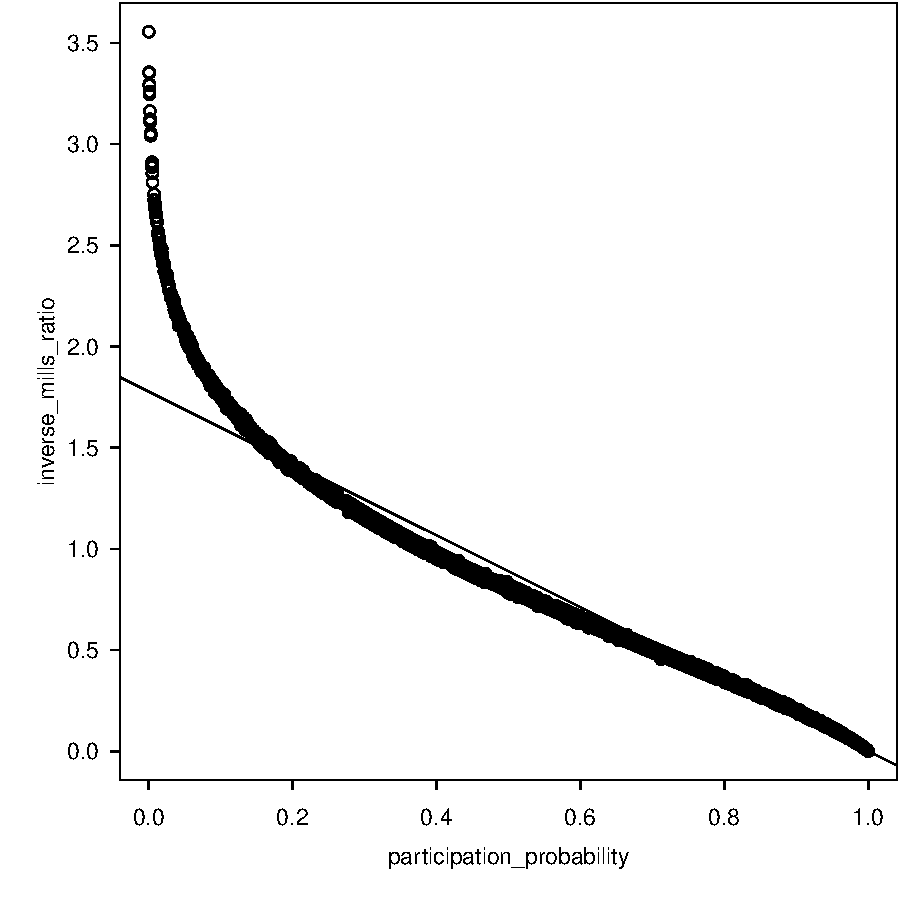
\includegraphics[width=.6\linewidth]{figure/script-Rnwauto-report-2} 

}


\begin{kframe}\begin{alltt}
\hlcom{# Draw the best fit line for the full sample.}
\hldef{best_fit_line_full_sample} \hlkwb{<-} \hlkwd{lm}\hldef{(inverse_mills_ratio}\hlopt{~}\hldef{participation_probability,} \hlkwc{data}\hldef{=dataset)}
\hlkwd{plot}\hldef{(inverse_mills_ratio}\hlopt{~}\hldef{participation_probability,} \hlkwc{data}\hldef{=dataset)}
\hlkwd{abline}\hldef{(}\hlkwc{a}\hldef{=}\hlkwd{coef}\hldef{(best_fit_line_full_sample)[}\hlnum{1}\hldef{],} \hlkwc{b}\hldef{=}\hlkwd{coef}\hldef{(best_fit_line_full_sample)[}\hlnum{2}\hldef{])}
\end{alltt}
\end{kframe}

{\centering \includegraphics[width=.6\linewidth]{figure/script-Rnwauto-report-3} 

}


\end{knitrout}


\end{document}
